\chapter{SELECTION OF THE REPRESENTATIVE SETS FROM THE EQUIVALENCE CLASSES OF
RNA CONTAINING 3D STRUCTURES}

\section{Introduction and motivation}

The previous chapter discussed a method for organizing all RNA IFE's extracted
from mmCIFs from PDB into sets of Equivalence Classes (EC). This procedure
organizes the 3D RNA structural dataset. However, for many use cases, simply
organizing the data is just the first step. In particular, studies exploring the
statistical properties of the structural data set will be biased toward 3D
structures that are highly represented in PDB, as is currently the case with
tRNA and ribosome structures. The number of highly populated EC's are compared in
Table~\ref{tab:mol-dist}.

\begin{table}
  \begin{tabulary}{\linewidth}{LRR}
    \toprule
    Molecule &
      Number of Integrated Functional Elements in the class &
      Percent of all RNA containing structures in PDB as of Sept 09, 2016 \\
    \midrule
    \TT{} LSU            & 282  & 4.0  \\
    \TT{} SSU            & 379  & 5.4  \\
    \TT{} 5S             & 282  & 4.0  \\
    \EC{} LSU            & 161  & 2.2  \\
    \EC{} SSU            & 157  & 2.2  \\
    \EC{} 5S             & 156  & 2.2  \\
    \HM{} LSU            & 69   & 0.9  \\
    \HM{} 5S             & 67   & 0.9  \\
    \DR{} LSU            & 42   & 0.5  \\
    \SC{} SSU            & 56   & 0.8  \\
    \SC{} LSU            & 63   & 0.9  \\
    % Other Ribosomes      &      &      \\
    Ribosomal Subtotal   & 1714 & 24.5 \\
    Remaining Structures & 5287 & 75.5 \\
    Total                & 7001 & 100  \\
    \bottomrule
  \end{tabulary}
  \caption{Proportion of solved structures that are from bacterial and yeast
    ribosomes. This table shows data from the 2.92 release of NR set at the
    ``all'' resolution, availabe at:
    \URL{http://rna.bgsu.edu/rna3dhub/nrlist/release/2.92/all}. This dataset contains
    all structures available as of Sept 09, 2016. This table presents the
    fraction of the total structural database that comprises structures from all
    sources ribosomes. In total they make up 20\% of the solved crystal
  structures. LSU: Large Ribosomal Subunit, SSU: Small Ribosomal Subunit.}
\label{tab:mol-dist}
\end{table}

As seen in the table, \EC{} and \TT{} rRNA make up 20\% of the entire dataset,
in terms of number of structures not nucleotides, and all rRNA from all species
total 24.5\%. For many statistical analyses of RNA structure, it is desirable to
identify one high quality representative IFE for each EC~\cite{Leontis2012b}.
For example, such a reduced redundancy dataset set is desirable for constructing
the RNA 3D Motif Atlas~\cite{Petrov2013}. In previous work, a method was
developed to identify representative structures from PDB format files; this set
was called the non-redundant (NR) set of RNA structures~\cite{Leontis2012b}. We
have updated the method to take advantage of the new mmCIF data format and to
overcome limitations of the previous method. The NR sets were posted
continously, on a weekly basis from February 5, 2011 to December 5, 2014 on the
BGSU RNA site and made available for searching on the NDB site
(\URL{http://ndbserver.rutgers.edu/}).

\section{Requirements for representative set}

The set of representative structures has a variety of uses in structural
bioinformatics applications. Most notably it supports the population and regular
updating of the RNA 3D Motif Atlas at \URL{http://rna.bgsu.edu/rna3dhub/motifs}.
The current version of the RNA 3D Motif Atlas is a clustering of all high
quality loops extracted from all structures in a recent Representative Set of
structures. For this reason it is desirable to avoid frequent changes in the
representative structure from release to release due to insignificant increments
in the selection criteria. If we allow frequent insignificant changes in the
representative structures selected for the Representative Set these changes
cause large changes in the RNA 3D Motif Atlas. This makes the resource appear
more unstable than it actually is and so we aim to avoid changes due to minor
improvements in structures. Thus the goals of the improvements described in
this chapter are:

\begin{enumerate}
  \item The Representative Set of structures should contain the highest quality
    representative X-Ray structures from each Equivalence Class. NMR or Cyro-EM
    structures are chosen as representatives only when no X-ray structure is
    available.

  \item The representative set should only change upon the appearance of new,
    significantly better structures, using criteria explained in this chapter.

  \item The representative set should reflect observed variation in sequence,
    structure, and biological variation in the set of EC's.
\end{enumerate}

The Representative Set (RS) is intended to display the observed structural,
sequence, and biological variation present in the current RNA-containing
structural dataset, avoiding duplication as much as possible. Each unique
structural class should be represented in the RS by one high quality structure,
as the EC already take into account the possibility of large structural
variation, as explained in the Chapter 3. It is desirable to pick the highest
quality IFE available from each EC\@. A high quality IFE is one that models the
experimental data as well or better than other available IFEs and is as complete
as possible.

\section{Methodology for selecting representative RNA 3D structures from
Equivalence classes}

This dissertation describes new methodology that represents significant
improvements over the previously developed methodologies for populating the RS
the BGSU RNA resource. In the previous method, the Representative Structure from
each Equivalence Class was selected based solely upon the number of annotated
base pairs per nucleotide caculated for each IFE, discussed in detail in
\cite{Leontis2012b}.

As the goal is to use only high quality structures, the procedure uses X-ray
structures as the representative, if possible. Some structures, such as that of
the mouse ribosome (3J7Q)~\cite{Voorhees2014}, have only been solved using
cryo-electron microscopy (``cryo-EM'') and in these cases, and only these cases,
the RS representative selected from that EC the equivalence set is necessarily a
cryo-EM structure. X-Ray structures are preferentially selected when available,
because methods for assessing the modeling quality of cryo-EM structures,
comparable to RSR-Z scores for X-ray crystallography are still under development
and are not yet available available (Helen Berman, personal communication).
Having objective assessment data, like RSR-Z scores available is essential for
downstream applications such as selecting reliable loops for inclusion in the
Motif Atlas. As soon as reliability data comparable to RSRZ scores are available
for cryo-EM structures, these structures will be treated on an equivalent
footing as X-ray structures.

The procedure for selecting RS from each EC containing more than one IFEs,
comprises theses steps:

\begin{enumerate}
  \item Select the structure with the highest number of annotated basepairs per
    nucleotide.

  \item search for all structures with at least 1\% more bases and base pairs and select
    it as the current representative

  \item Repeat step 2 until there no structure has more base pairs and bases.
\end{enumerate}

This procedure has a few features that are worth discussing in detail. First, we
use the number of FR3D annotated base pairs per nucleotide (BP/NT) as the
measure of structural quality, because in our experience a high quality model of
the same RNA molecule contains more annotated base pairs of all types than a
poor model. This is a useful proxy and not a direct measure of the modeling
quality such as that provided by Real Space Refinement (RSR) statistics which is
provided now by PDB for all structures. RSR measures how well a structural model
fits the underlying experimental electron density and is discussed in more
detail in the next chapter, where I use it to filter 3D loops.

Secondly, this method is designed to select a structure based both on the value
of BP/NT but also the total number of nucleotides in the IFE\@. Structures in the
same EC vary in the number of resolved nucleotides as discussed in Chapter 3. If
we use only BP/NT then we may select a  smaller structure that omits parts of
the 3D structure that are less well modeled. We prefer more complete
representative structures over smaller structures and thus include this second
criterion.

Finally, the new method requires new representatives to show a significant
increase in both the number of nucleotides and the BP/NT to become the
representative. By doing so, we avoid changing representatives upon
insignificant changes in overall quality, thus stabilizing the RS over time.
This 1\% increase is an empirically determined threshold that may be adjusted in
the future. The new method of representative selection described in this
dissertation will be referred to henceforth as the ``dual 1\% increase'' method.
I have also created a method called the ``any increase'' method which does not
have require a 1\% increase in basepairs and nucleotides for switching
representative. This method is created for comparison to examine the effect of
the 1\% threshold.

To describe the overall logic of the method I have added a figure of the
pseudocode in Figure~\ref{fig:pseudocode-cur-representatives}. This figure shows
the overall logic of this procedure, but does not correspond exactly to the
implementation, as the implementation contains much more error handling logic.
It is important to note that while this logic does not directly consider the
previous representative it does appear to be stable, as discussed below.
However, a small modification to the procedure as shown in
Figure~\ref{fig:pseudocode-new-representatives} would.

\begin{figure}
  \begin{subfigure}[b]{0.5\textwidth}
    \begin{tabbing}
      proc\=edur\=e sel\=ecting a representative \\
      \>select candidate representative with best BP/NT \\
      \>for all members of the group \\
        \>\>If representative has 1\% more BP and 1\% NT \\
          \>\>\>set as representative \\
          \>\>End \\
        \>End \\
      \>repeat loop until representative does not change \\
      End
    \end{tabbing}
    \caption{Current representative selection}
\label{fig:pseudocode-cur-representatives}
  \end{subfigure}
  \begin{subfigure}[b]{0.5\textwidth}
    \begin{tabbing}
      proc\=edur\=e sel\=ecting a representative \\
      \>select candidate representative which is previous representative \\
      \>for all members of the group \\
        \>\>If representative has 1\% more BP and 1\% NT \\
          \>\>\>set as representative \\
          \>\>End \\
        \>End \\
      \>repeat loop until representative does not change \\
      End
    \end{tabbing}
    \caption{Possible new representative selection}
\label{fig:pseudocode-new-representatives}
  \end{subfigure}
  \caption{Pseudocode showing the overall logic of the selection for
  representative sets.}
\label{fig:pseudocode-representatives}
\end{figure}

\section{Results of building the representative set}

I evaluated the RS selected as described above by using the new
dual 1\% increase method, and compared results with the previous method and a
modification of the current method that changes the representative structure
based upon improvement of just one criterion. These classes used all available
structures from July 28, 2016. I will first discuss the differences between
structures selected by these methods and then move on to to examine the
stability of the methods.

\subsection{Selection of Structures for the Representative Set}

I evaluated the selection of representatives by examining the selection of
representatives from the equivalence classes built in the previous chapter. This
used all structures available as of July 25, 2016 (equivalent to release 2.86).
I examined classes for changes and determined where the new method selected
different representatives than the other methods. These changes were then
examined manually to assess the quality of the structures using the original as
well as additional criteria. There were 29 classes in the data set for which
different representatives were selected by the two methods. Shown in
Figure~\ref{fig:hm-lsu-rep} is a summary of the representative selection for the
three methods discussed here. The upper panel shows the previous method where we
can see the structure that is at the top of stack of very similar structures is
selected as the representative. This contrasts with our 1\% increase method which
selects a example with more nucleotides and basepairs but a worse ratio of the
two. This selection is our desired result.

\begin{figure}
  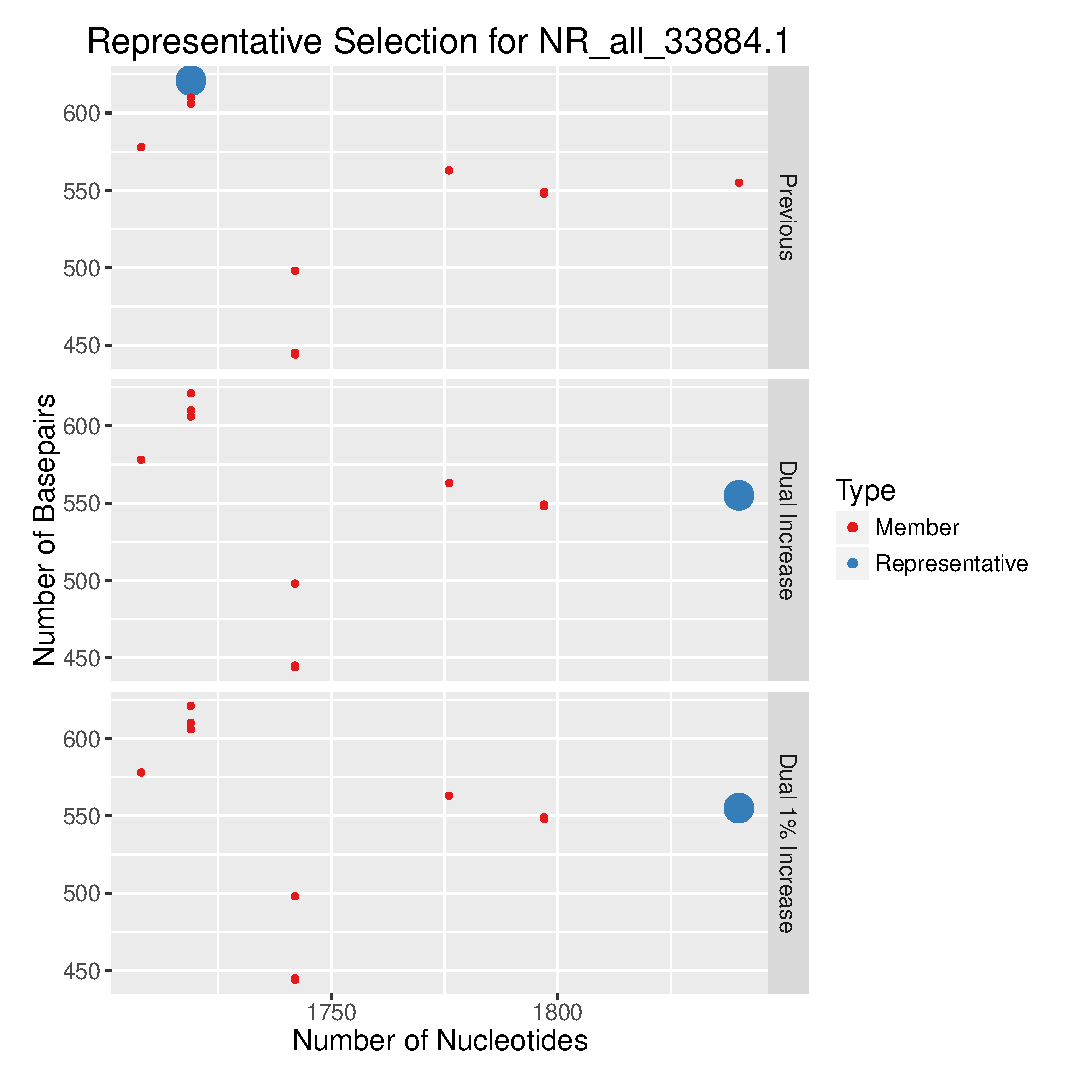
\includegraphics[width=0.5\textwidth]{chapter-4/figs/hm-lsu-rep}
  \caption{Scatter plot of representative selection across three possible
    methodologies for the \HM{} Large Ribosomal Subunit. Shown here is a summary
    of which IFE’s are selected as the representative for the three method discussed
    here. Each panel indicates a different method, in order from top to bottom,
    the previous method based only on BP/NT criterion, the Dual 1\% increase
    method and the any increase method. The representative IFE is colored in
    blue, while the other members of the set are colored red. The upper panel
    shows the previous method. It is difficult to see but the IFE selected as
    the representative is the IFE at the top of the stack of IFE’s in the upper
    right.}
\label{fig:hm-lsu-rep}
\end{figure}

We then evaluated the selection of representative in context of the resolution
distribution. The ideal selection has the highest resolution of any structure in
the class. Show in Figure~\ref{fig:hm-rep-res-dist} is a summary. In it we can
see that all three methods select an IFE with resolution 2.4{\AA}. This is
consistent with our goals for the methods.

\begin{figure}
  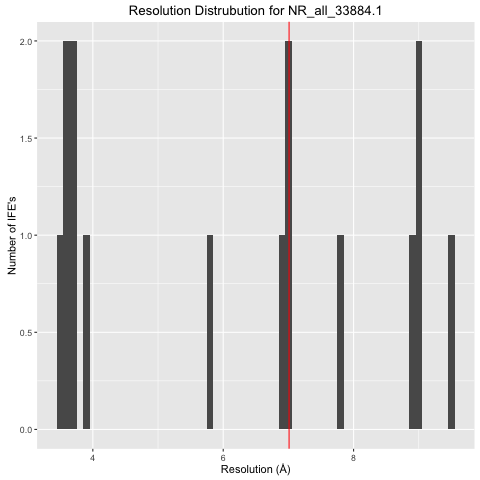
\includegraphics[width=0.5\linewidth]{chapter-4/figs/hm-lsu-res}
  \caption{Distribution of resolutions for \HM{} Large Ribosomal subunit IFE’s
    in NR\_all\_65634.1 with the resolution of the representative indicated.
    This histogram shows the resolution distribution of all IFE’s in the
    class. The red line indicates the resolution of the representative chosen by
  all 3 methods.}
\label{fig:hm-rep-res-dist}
\end{figure}

We further evaluated the method described here by examining the selection of
representatives for the \EC{} Large and Small Subunits as well as the \TT{}
Large and Small Ribosomal Subunits, shown in Figure~\ref{fig:ec-lsu-rep},
Figure~\ref{fig:ec-ssu-rep}, Figure~\ref{fig:tt-lsu-rep} and
Figure~\ref{fig:tt-ssu-rep} respectively. As we can see in these figures, only
the \EC{} LSU \TT{} SSU differ in selection of representatives.

\begin{figure}
  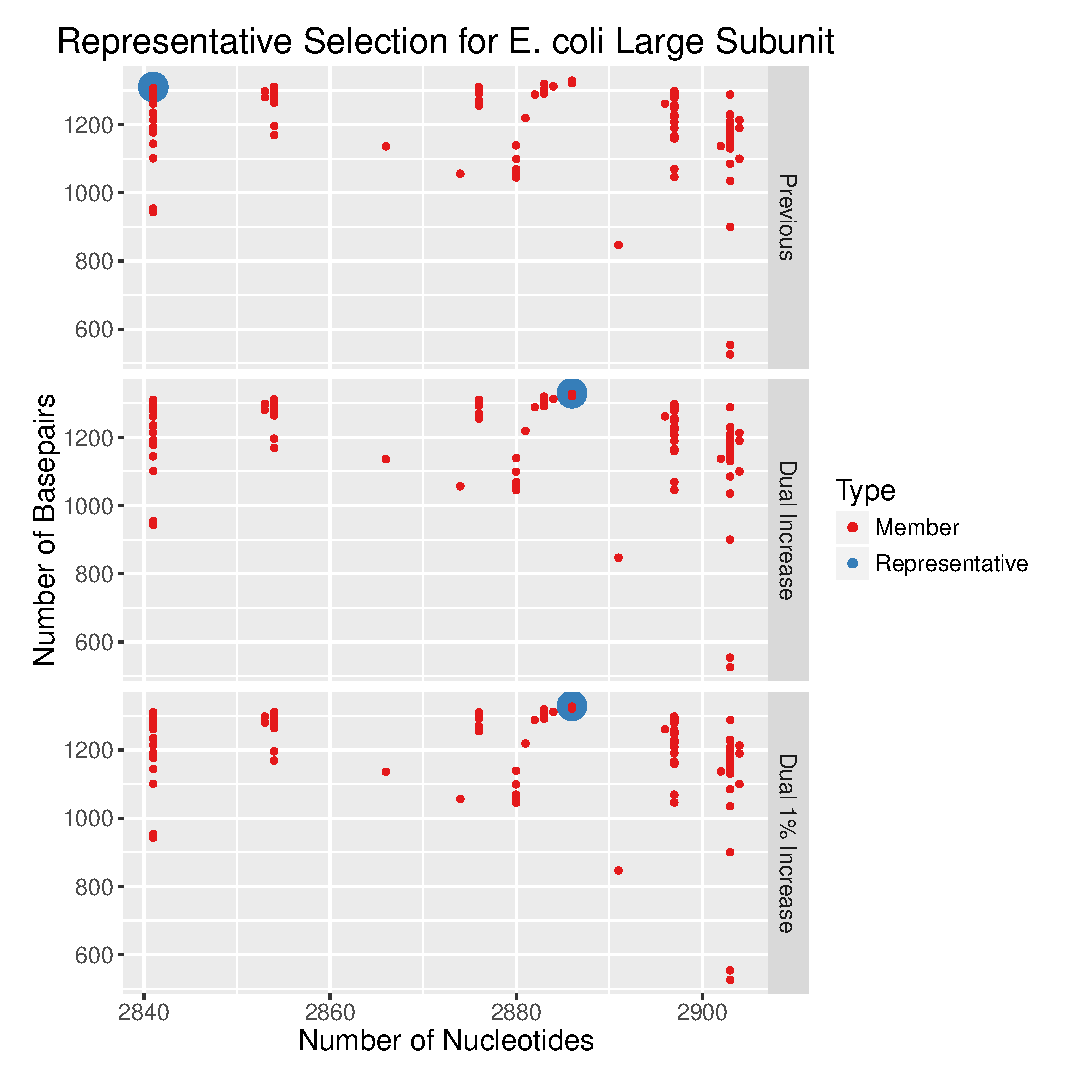
\includegraphics[width=0.5\linewidth]{chapter-4/figs/ec-lsu-rep}
  \caption{Scatter plot of the number of base pairs vs the number of nucleotides
    for selected \EC{} LSU rRNAs using the three methods discussed here.
    The representative selected is shown as a large blue dot, while all other
    members are shown as small red dots. The plot has been truncated to show
    only the structures with at least 2840 nucleotides and 500 basepairs for
  relevance.}
\label{fig:ec-lsu-rep}
\end{figure}

\begin{figure}
  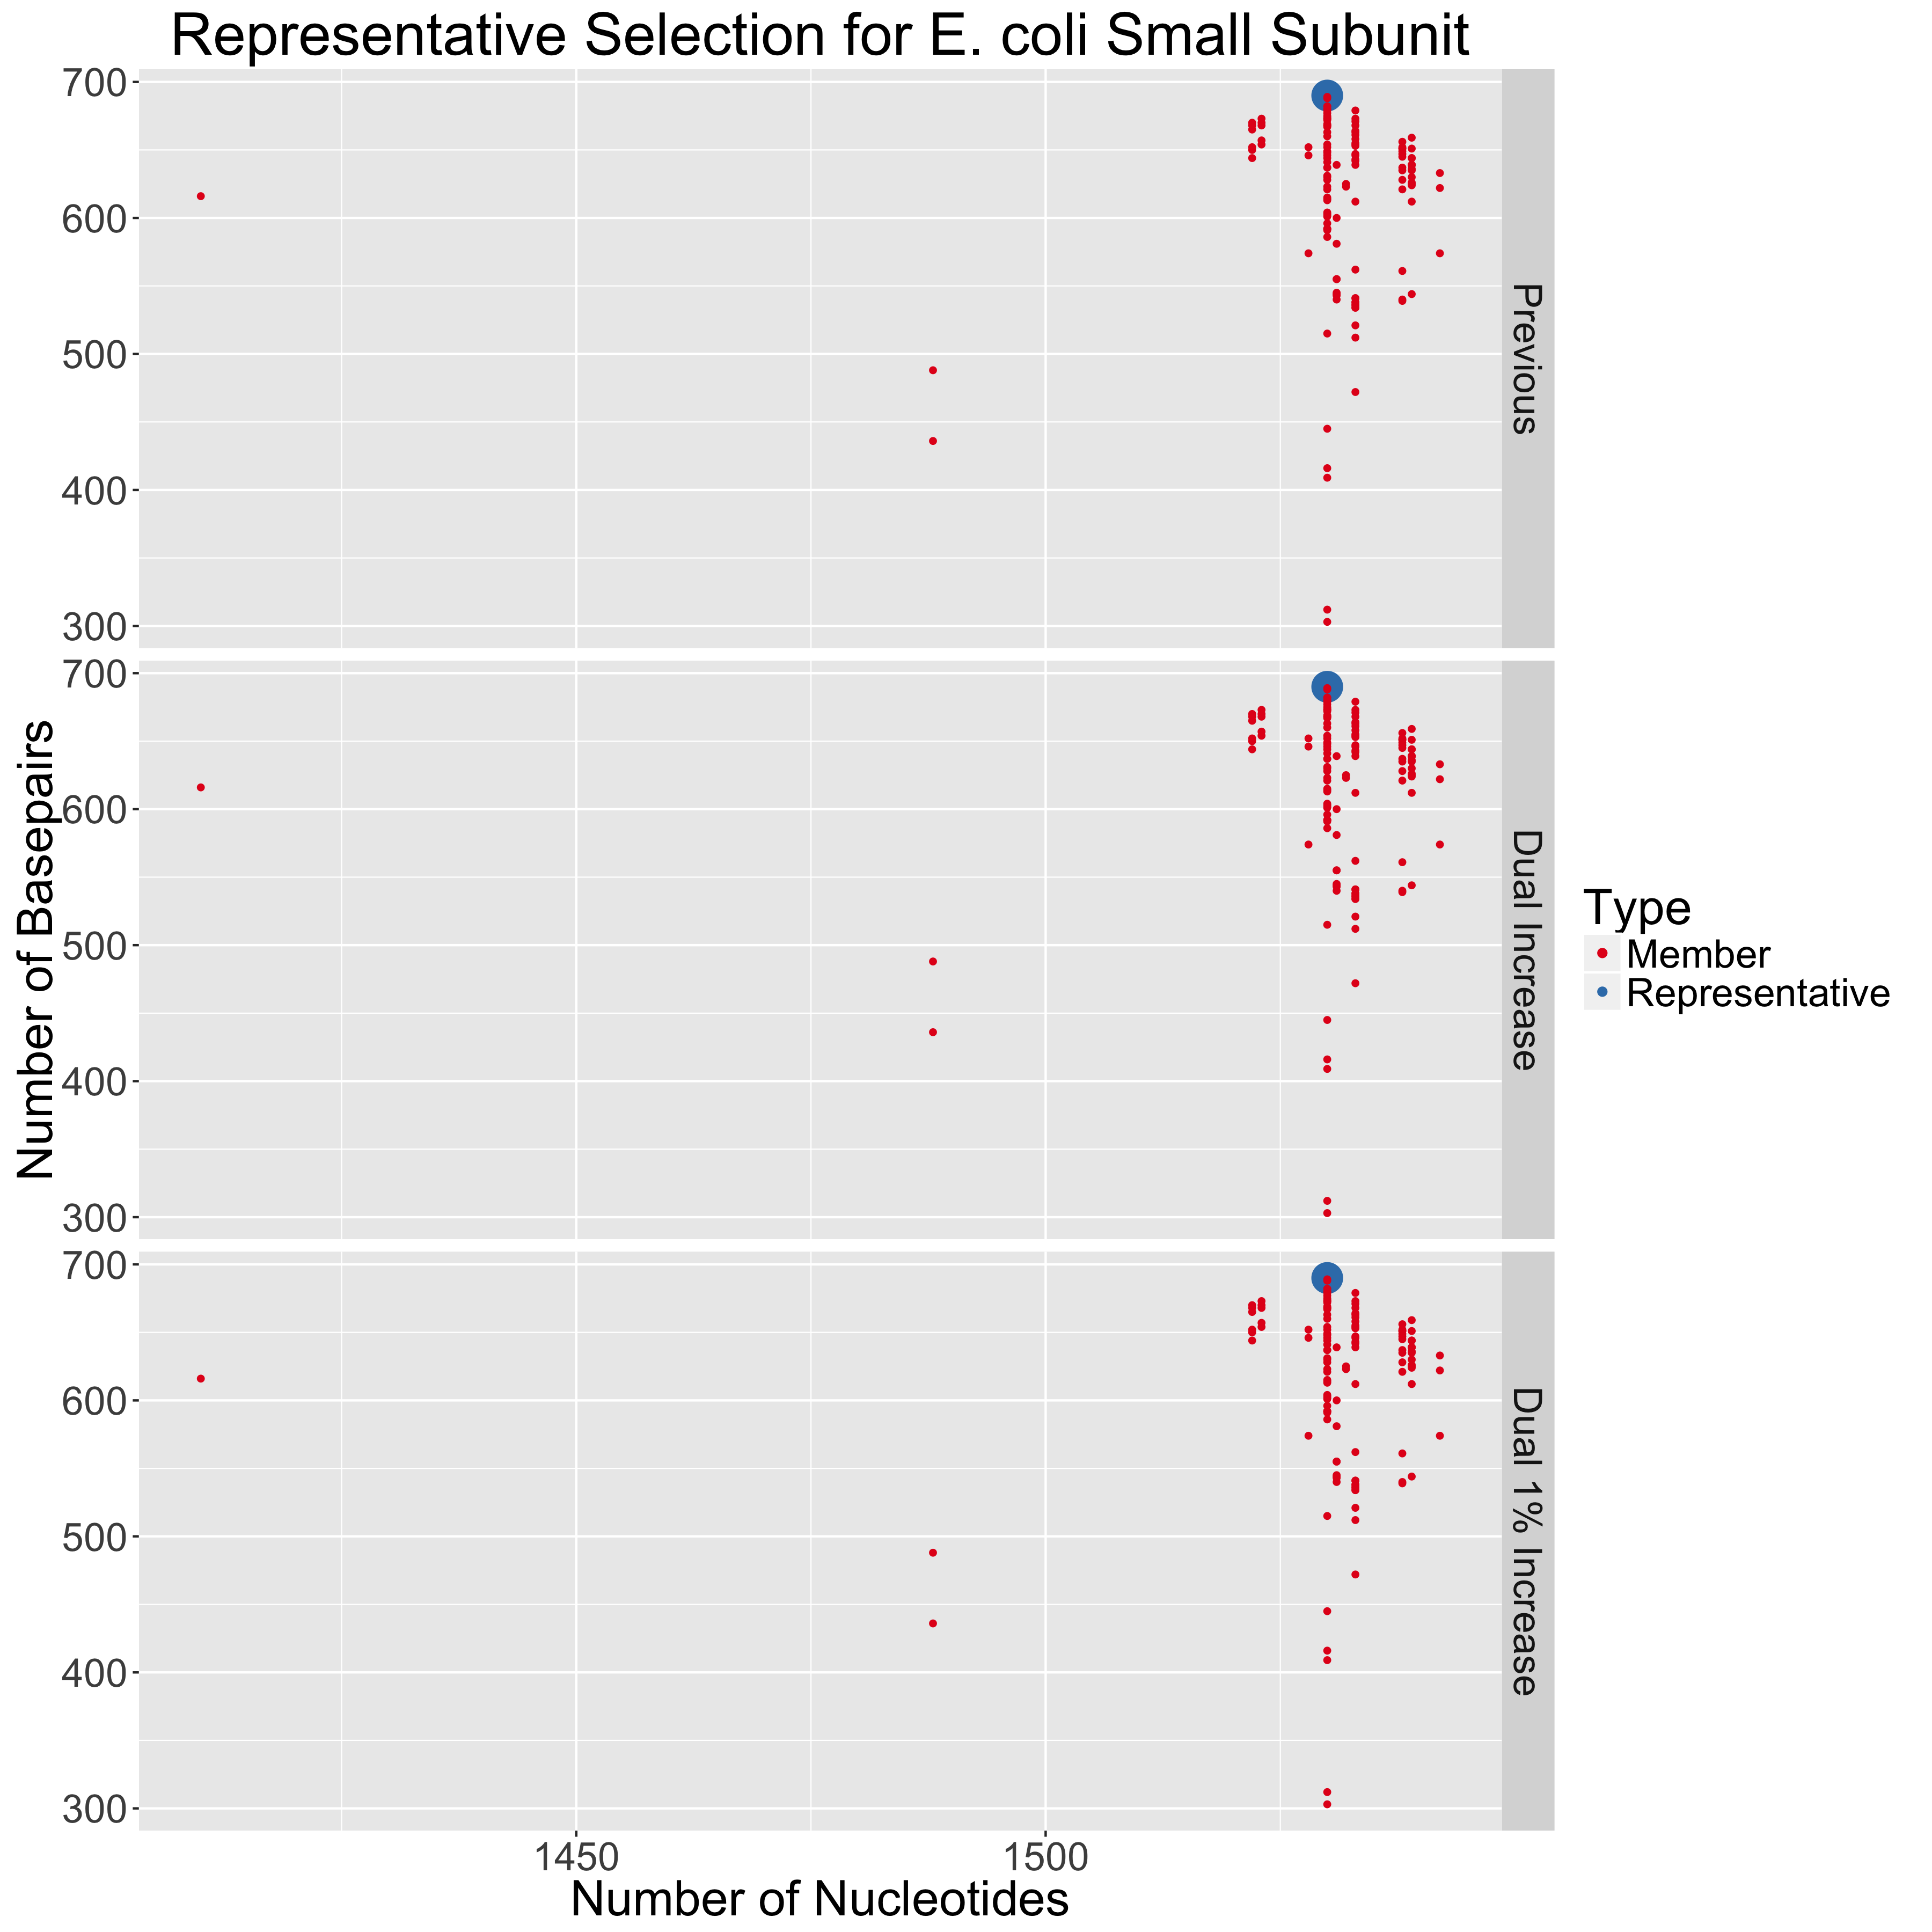
\includegraphics[width=0.5\linewidth]{chapter-4/figs/ec-ssu-rep}
  \caption{Scatter plot of the number of base pairs vs the number of nucleotides
    for selected \EC{} Small Subunits using the three methods discussed here.
    The representative selected is shown as a large blue dot, while all other
    members are shown as small red dots. The plot has been truncated to show
    only the structures with at least 1400 nucleotides and 300 basepairs for
  clarity.}
\label{fig:ec-ssu-rep}
\end{figure}

\begin{figure}
  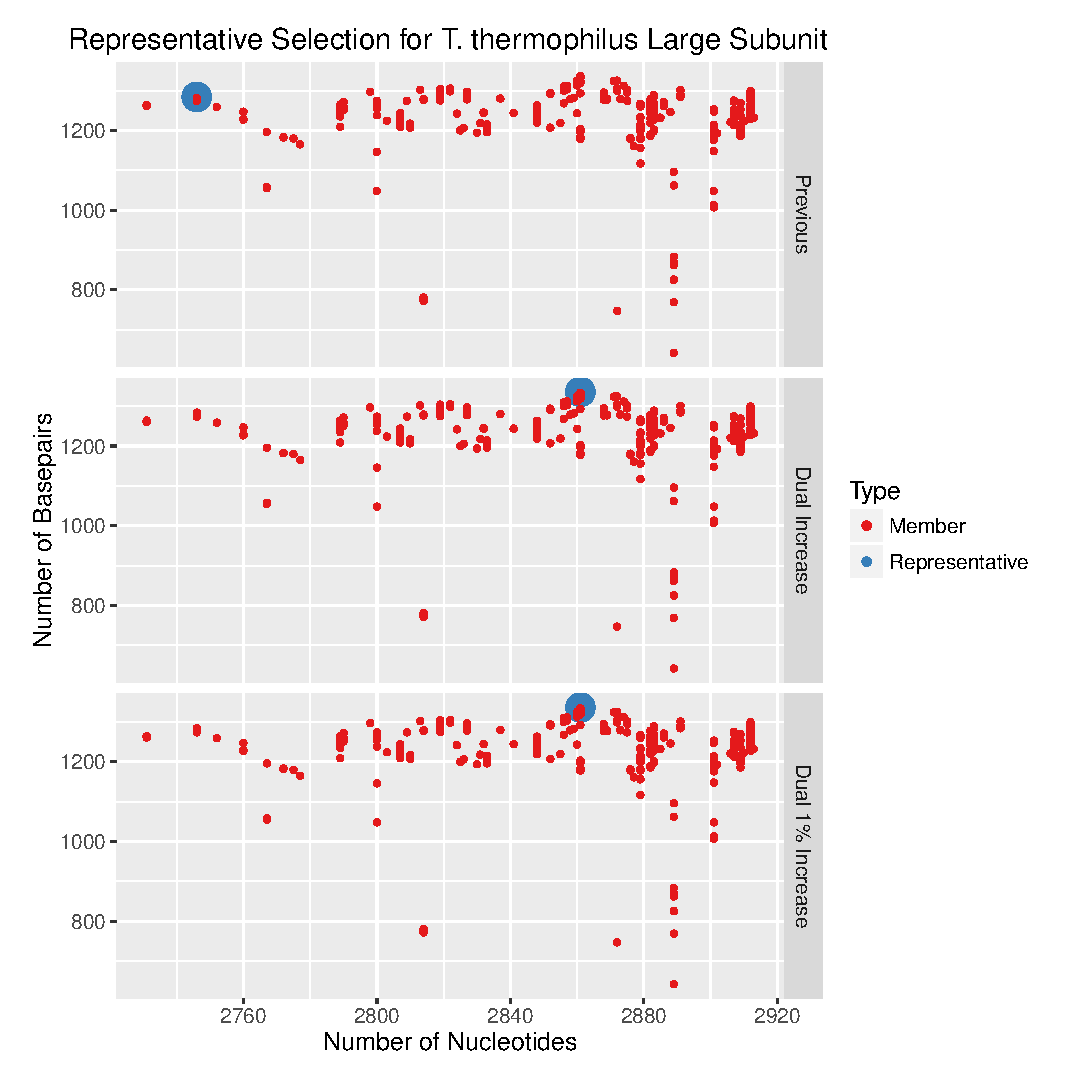
\includegraphics[width=0.5\linewidth]{chapter-4/figs/tt-lsu-rep}
  \caption{Scatter plot of the number of base pairs vs the number of nucleotides
    for selected \TT{} Large Subunits using the three methods
    discussed here. The representative selected is shown as a large blue dot,
    while all other members are shown as small red dots. The plot has been
    truncated to show only the structures with at least 2725 nucleotides and 500
  basepairs for clarity.}
\label{fig:tt-lsu-rep}
\end{figure}

\begin{figure}
  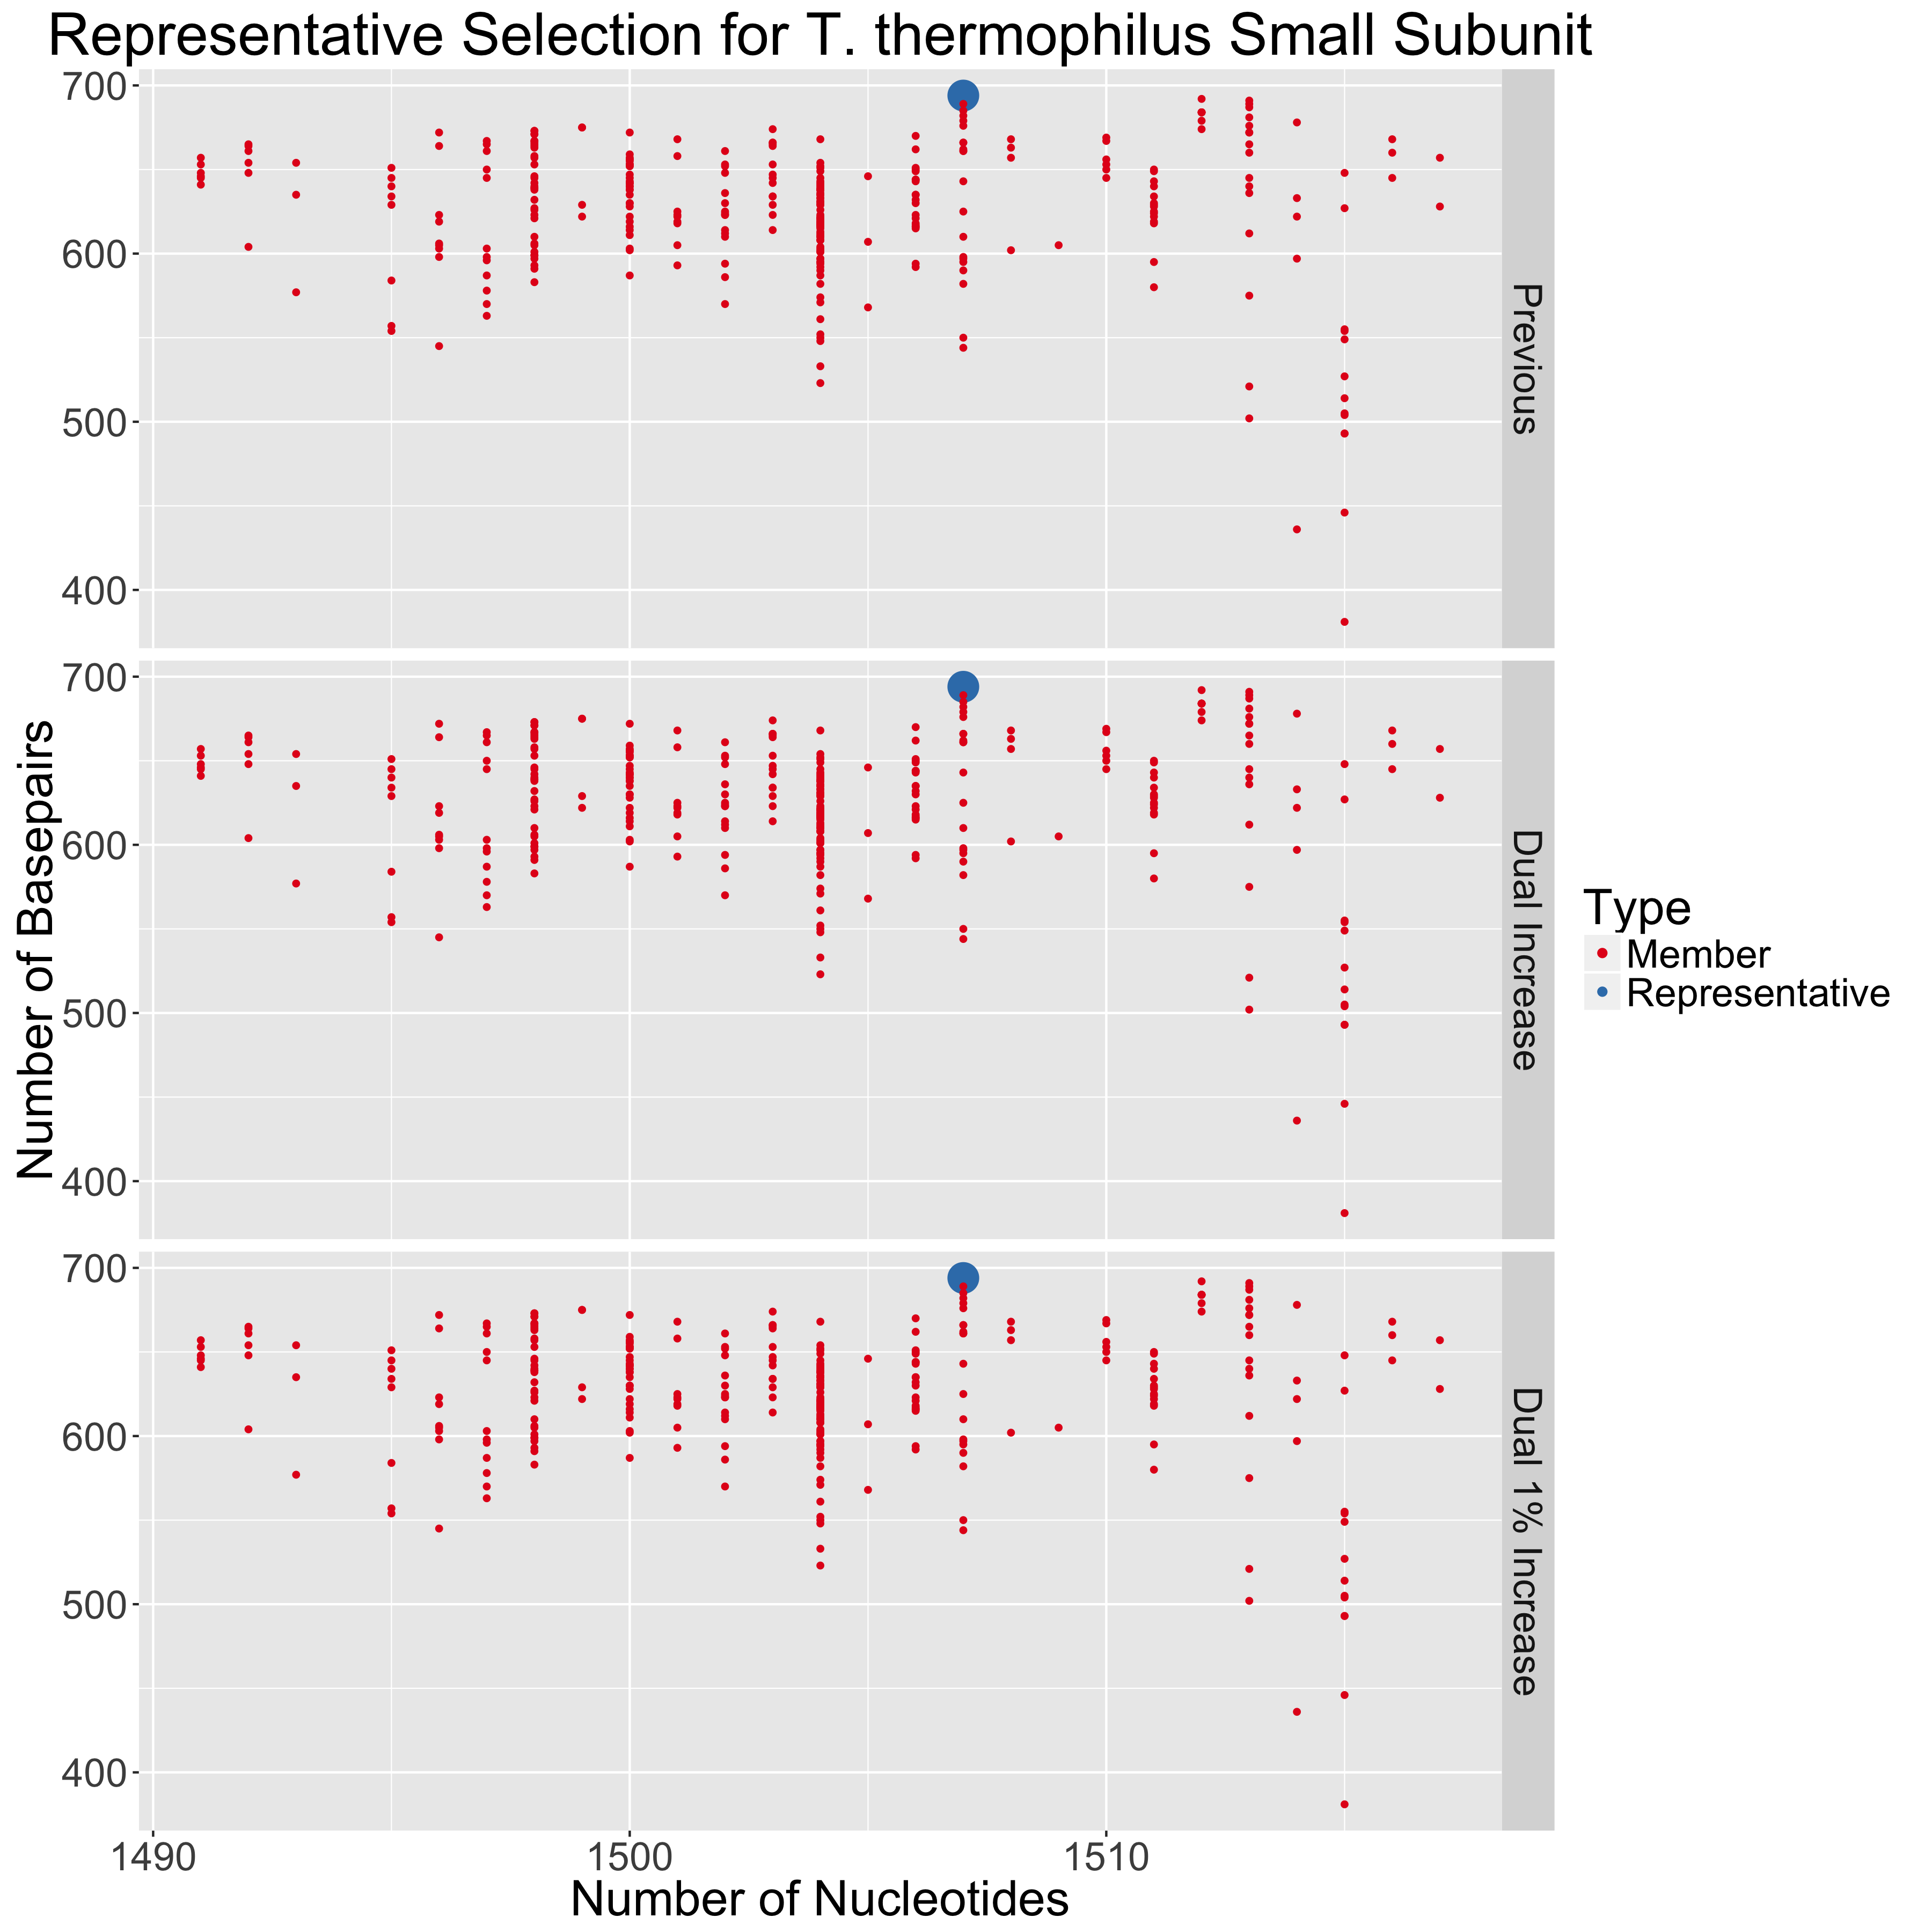
\includegraphics[width=0.5\linewidth]{chapter-4/figs/tt-ssu-rep}
  \caption{Scatter plot of the number of base pairs vs the number of nucleotides
    for selected \TT{} Small Subunits using the three methods
    discussed here. The representative selected is shown as a large blue dot,
    while all other members are shown as small red dots. The plot has been
    truncated to show only the structures with at least 1490 nucleotides and 200
  basepairs for clarity.}
\label{fig:tt-ssu-rep}
\end{figure}

\subsubsection{Evaluating representative selection on the basis of resolution}

Another useful criteria for evaluation our representative selection is to
examine if our method selects the structure with lowest resolution. Generally,
higher resolution structures are better than lower resolution structures. To
explore this I computed the difference between the selected representative for
all groups and the structure in the group with the smallest resolution. A
summary of this data is shown in Table~\ref{tab:res-diff-summary}.

\begin{table}
  \begin{tabulary}{\linewidth}{LRRR}
    \toprule
    Method &  Representatives with lowest resolution &  Representatives with
    resolution within 1{\AA{}}  & Representatives with resolution \textgreater 1{\AA} \\
    \midrule
    Previous          & 1506 (93\%) & 86 (5.3\%) & 14 (0.8\%) \\
    Dual Increase     & 1494 (93\%) & 97 (6.0\%) & 15 (0.9\%) \\
    Dual 1\% Increase & 1506 (93\%) & 88 (5.4\%) & 12 (0.7\%) \\
    \bottomrule
  \end{tabulary}
  \caption{A summary of the differences between the resolution of the
  representatives as compared to the member of the group with the lowest
  resolution.}
\label{tab:res-diff-summary}
\end{table}

From this we can see that nearly all groups use a structure with the lowest
resolution, as we desired. However, roughly 5\% of all groups have a
representative with resolution with 1{\AA} of the minimum. This leaves a very small
percent, less than 1\%, of all groups that use a representative with resolution
greater than 1{\AA} from the minimum. Shown in Figure~\ref{fig:res-diff-histogram}
is a histogram that displays the differences for all groups where the difference
is greater than 0{\AA}.

\begin{figure}
  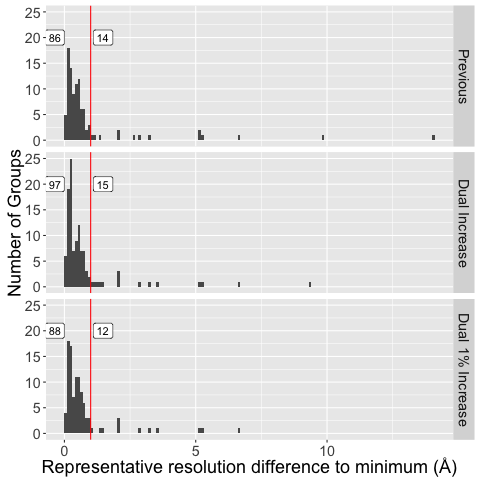
\includegraphics[width=0.5\linewidth]{chapter-4/figs/res-diff}
  \caption{Histogram of the differences between the resolution of the selected
    representative and the minimum resolution within the group for all 3
    methods. This histogram does not show the groups where the representative
    resolution is the same as the minimum resolution.  The red vertical line
    indicates the cutoff of 1{\AA}. The numbers to the left of the red box indicate
    the total number of groups with resolution difference less than 1{\AA}, while
    the number to the right indicates the number of groups with resolution
  difference greater than 1{\AA}.}
\label{fig:res-diff-histogram}
\end{figure}

From this figure we can see two things. First, all methods are very similar in
terms of the number of groups that select representatives with unusually high
resolution. Secondly, several groups have very large differences between the
selected representative and the minimum resolution. For example one group has a
difference of 14\AA. Examining this data shows that there are 19 groups with
resolution differences. Shown in Table~\ref{tab:rep-res-diff-details} are the
summary of those groups.

\begin{landscape}
  \begin{table}
  \begin{tabular}{llrrr}
    \toprule
               &                             & \multicolumn{3}{c}{Method} \\
    \cmidrule(r){3-5}
    Group Name &  Minimum Resolution ({\AA}) &  Previous &  Dual Increase &  Dual 1\% Increase \\
    \midrule
    NR\_all\_00304.1 &  9.0  & \ife{3J0D}{1}{A} (11.1{\AA})   &
                               \ife{3J0D}{1}{A} (11.1{\AA})   &
                               \ife{3J0D}{1}{A} (11.1{\AA})   \\
    NR\_all\_13601.2 &  5.0  & | & 
                               \ife{4KZZ}{1}{j} (7.03{\AA})  &
                               \ife{4KZZ}{1}{j} (7.03{\AA})  \\
   NR\_all\_14586.1 &  3.5  & | & 
                              \ifePair{4V6X}{1}{A5}{4V6X}{1}{A8} (5{\AA})  &
                              \ifePair{4V6X}{1}{A5}{4V6X}{1}{A8} (5{\AA}) \\
    NR\_all\_16577.1 &  6.9  & \ife{3J0O}{1}{V} (9{\AA})  &
                               \ife{3J0O}{1}{V} (9{\AA})  &
                               \ife{3J0O}{1}{V} (9{\AA})  \\
    NR\_all\_18070.1 &  2.4  & | & 
                               \ife{4TUD}{1}{QV} (3.6{\AA}) & 
                               | \\
    NR\_all\_33599.2 &  2.6  & \ife{4V5M}{1}{AV} (7.8{\AA}) &
                               | &
                               | \\
    NR\_all\_33884.1 &  3.45 & | & 
                               \ife{4KZY}{1}{i} (7.01{\AA})  &
                               \ife{4KZY}{1}{i} (7.01{\AA}) \\
    NR\_all\_37074.2 &  2.1  & \ife{4V6Z}{1}{BB} (12{\AA})   &
                               \ife{5J88}{1}{DB} (3.32{\AA}) &
                               | \\
    NR\_all\_39327.1 &  3.8  & \ife{4V6M}{1}{AV} (7.1{\AA})  &
                               \ife{4V6M}{1}{AV} (7.1{\AA})  &
                               \ife{4V6M}{1}{AV} (7.1{\AA})  \\
    NR\_all\_39428.1 &  2.6  & \ife{4V8U}{1}{CV} (3.7{\AA})  &
                               \ife{4V8U}{1}{CV} (3.7{\AA})  &
                               \ife{4V8U}{1}{CV} (3.7{\AA})  \\
    NR\_all\_44399.2 &  2.96 & \ife{4V70}{1}{A1} (17{\AA}) & 
                               | & 
                               | \\
    NR\_all\_48374.2 &  2.1  & \ife{1C04}{1}{F} (5{\AA})  &
                               \ife{1C04}{1}{F} (5{\AA})  &
                               \ife{1C04}{1}{F} (5{\AA})  \\
    NR\_all\_55323.1 &  3.71 & \ife{4V68}{1}{AY} (6.4{\AA}) &
                               | & 
                               | \\
    NR\_all\_59913.2 &  2.1  & \ife{4V4Q}{1}{CA} (3.46{\AA})  &
                               \ife{4V4Q}{1}{CA} (3.46{\AA})  &
                               \ife{4V4Q}{1}{CA} (3.46{\AA})  \\
    NR\_all\_62116.2 &  2.1  & \ife{4V54}{1}{DB} (3.3{\AA})   &
                               | & 
                               | \\
    NR\_all\_68375.1 &  8.3  & \ife{3IZ4}{1}{A} (13.6{\AA})  &
                               \ife{3IZ4}{1}{A} (13.6{\AA})  &
                               \ife{3IZ4}{1}{A} (13.6{\AA})  \\
    NR\_all\_87281.1 &  3.9  & | & 
                               \ife{3J3V}{1}{B} (13.3{\AA})   &
                               | \\
    NR\_all\_95973.1 &  3.8  & \ife{4D61}{1}{j} (9{\AA})  &
                               \ife{4D61}{1}{j} (9{\AA})  &
                               \ife{4D61}{1}{j} (9{\AA})  \\
    NR\_all\_97012.1 &  2.0  & \ife{4V49}{1}{AW} (8.7{\AA})  &
                               \ife{4V49}{1}{AW} (8.7{\AA})  &
                               \ife{4V49}{1}{AW} (8.7{\AA})  \\
    \bottomrule
  \end{tabular}
  \caption{Listing of all groups that do not use the structure with the lowest
  representative for all representative selection methods. This table shows all
groups where at least one method does not use a structure with the lowest
resolution for one method. The ``|'' indicates that the method selects a
structure with the given resolution. The minimum resolution for the group is
shown along with the group id. For each method column the IFE selected is shown
and the resolution for the IFE is shown in parenthesis. }
\label{tab:rep-res-diff-details}
  \end{table}
\end{landscape}

The new method will not select a cryo-EM structure if an X-ray structure is
available, however, new cryo-EM structure are being solved with increasingly
higher accuracy, rapidly approaching the quality of X-ray structures. This is a
potential reason for the differences found in Table~\ref{tab:rep-res-diff-details}.
I examined this by determining the difference between the resolution of the
representative structure and the minimal resolution in that group for all
groups, using only X-ray structures and repeating the analysis. Shown in
Figure~\ref{fig:xray-only-diff} is this figure.

\begin{figure}
  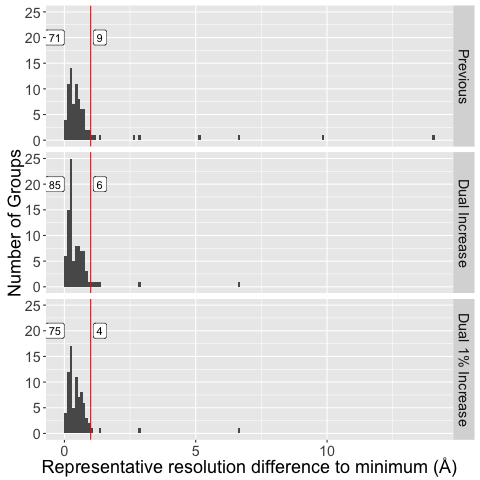
\includegraphics[width=0.5\linewidth]{chapter-4/figs/xray-res-diff}
  \caption{Histogram of the differences between the resolution of the selected
    representative and the minimum resolution for X-Ray structures within the
    group for all 3 methods. This histogram does not show the groups where the
    representative resolution is the same as the minimum resolution.  The red
    vertical line indicates the cutoff of 1{\AA}. The numbers to the left of the
    red box indicate the total number of groups with resolution difference less
    than 1{\AA}, while the number to the right indicates the number of groups
    with resolution
  difference greater than 1{\AA}.}
\label{fig:xray-only-diff}
\end{figure}

In this figure we can see that there are very few groups have resolution
difference greater than 1\AA{} for all methods. As with the previous analysis, all
methods perform similarly in terms of the number of groups with large
differences. However, the Dual 1\% method does show a smaller resolution
difference. Shown in Table~\ref{tab:xray-only-outliers} are the groups with large
difference between the representative resolution and minimum resolution.

\begin{landscape}
\begin{table}
  \begin{tabular}{llrrr}
    \toprule
          &                             & \multicolumn{3}{c}{Method} \\
    \cmidrule(r){3-5}
    Group &  Minimum Resolution ({\AA}) & Previous &  Dual Increase  & Dual 1\% Increase \\
    \midrule
    NR\_all\_18070.1 & \ife{4W2F}{1}{AX} (2.4{\AA}) & 
                       | & 
                       \ife{4TUD}{1}{QV} (3.6{\AA}) & 
                       | \\
    NR\_all\_33599.2 & \ife{5J8B}{1}{x} (2.6{\AA}) & 
                       \ife{4V5M}{1}{AV} (7.8{\AA}) & 
                       | &
                       | \\
    NR\_all\_37074.2 & \ife{4YBB}{1}{DB} (2.1{\AA}) & 
                       \ife{4V6Z}{1}{BB} (12{\AA}) & 
                       | &
                       | \\ 
    NR\_all\_39428.1 & \ife{5J8B}{1}{w} (2.6{\AA}) & 
                       \ife{4V8U}{1}{CV} (3.7{\AA}) & 
                       \ife{4V8U}{1}{CV} (3.7{\AA}) & 
                       \ife{4V8U}{1}{CV} (3.7{\AA})  \\
    NR\_all\_44399.2 & \ife{5IBB}{1}{3L} (2.96{\AA}) & 
                       \ife{4V70}{1}{A1} (17{\AA}) &
                       | & 
                       | \\
    NR\_all\_48374.2 & \ife{430D}{1}{A} (2.1{\AA}) & 
                       \ife{1C04}{1}{F} (5{\AA}) & 
                       \ife{1C04}{1}{F} (5{\AA}) & 
                       \ife{1C04}{1}{F} (5{\AA})  \\
    NR\_all\_55323.1 & \ife{4V4I}{1}{0} (3.71{\AA}) & 
                       \ife{4V68}{1}{AY} (6.4{\AA})  & 
                       | & 
                       | \\
    NR\_all\_59913.2 & \ife{4YBB}{1}{AA} (2.1{\AA}) &
                       \ife{4V4Q}{1}{CA} (3.46{\AA}) & 
                       \ife{4V4Q}{1}{CA} (3.46{\AA}) &
                       \ife{4V4Q}{1}{CA} (3.46{\AA}) \\
    NR\_all\_62116.2 & \ife{4YBB}{1}{DA} (2.1{\AA}) &
                       | &
                       | &
                       | \\
   NR\_all\_97012.1 & \ife{1EVV}{1}{A} (2{\AA}) &
                      \ife{1EVV}{1}{A} (2{\AA}) &
                      \ife{1EVV}{1}{A} (2{\AA}) &
                      \ife{1EVV}{1}{A} (2{\AA}) \\
    \bottomrule
  \end{tabular}
  \caption{Details of X-ray only groups without that do not have a
  representative with the minimum resolution. This table lists all groups where
at least one of the methods selects a representative that does not have the
highest resolution among the available structures. This table only contains
groups that contain only X-ray only. The ``|'' indicates that the method does
pick a structure with the minimum resolution.}
\label{tab:xray-only-outliers}
\end{table}
\end{landscape}

From this table we can see that the Dual 1\% increase has the fewest differences.
In addition, the times it does have issues are the same as the previous method,
indicating this method is not making new mistakes.

Overall, I note that the new method, Dual 1\% Increase, almost always, greater
than 90\% of the time, selects a representative that has a resolution close to
the best nominal resolution in the group. This is desirable because higher
resolution generally means a better structure. However, there are very few cases
w’here this does not occur. The new method performs better than the previous
version as there are fewer of these cases and the difference in resolution is
smaller. Many of these cases appear to be due to the group containing both
cryo-em and x-ray structures. The new method, by construction, will always
prefer X-ray structures, even when the nominally higher resolution is a cryo-EM
structure.

\subsubsection{Independent measures of representative selection}

PDB provides quality reports for all structures~\cite{Gore2012}. These quality
reports use a variety of metrics that were suggested by the X-ray validation
task force~\cite{Gore2012}. Here I evaluate our selection on the basis of data
from these quality reports. Shown in Figure~\ref{fig:ec-lsu-report} is the
quality report for the representative selected by the dual 1\% increase method
as compared to that of the previous method. From this figure we can see that the
dual 1\% increase method selects structures with fewer RSRZ outliers and similar
RNA backbone scores, however, all other metrics are worse.

\begin{figure}
  \begin{subfigure}[b]{0.5\textwidth}
    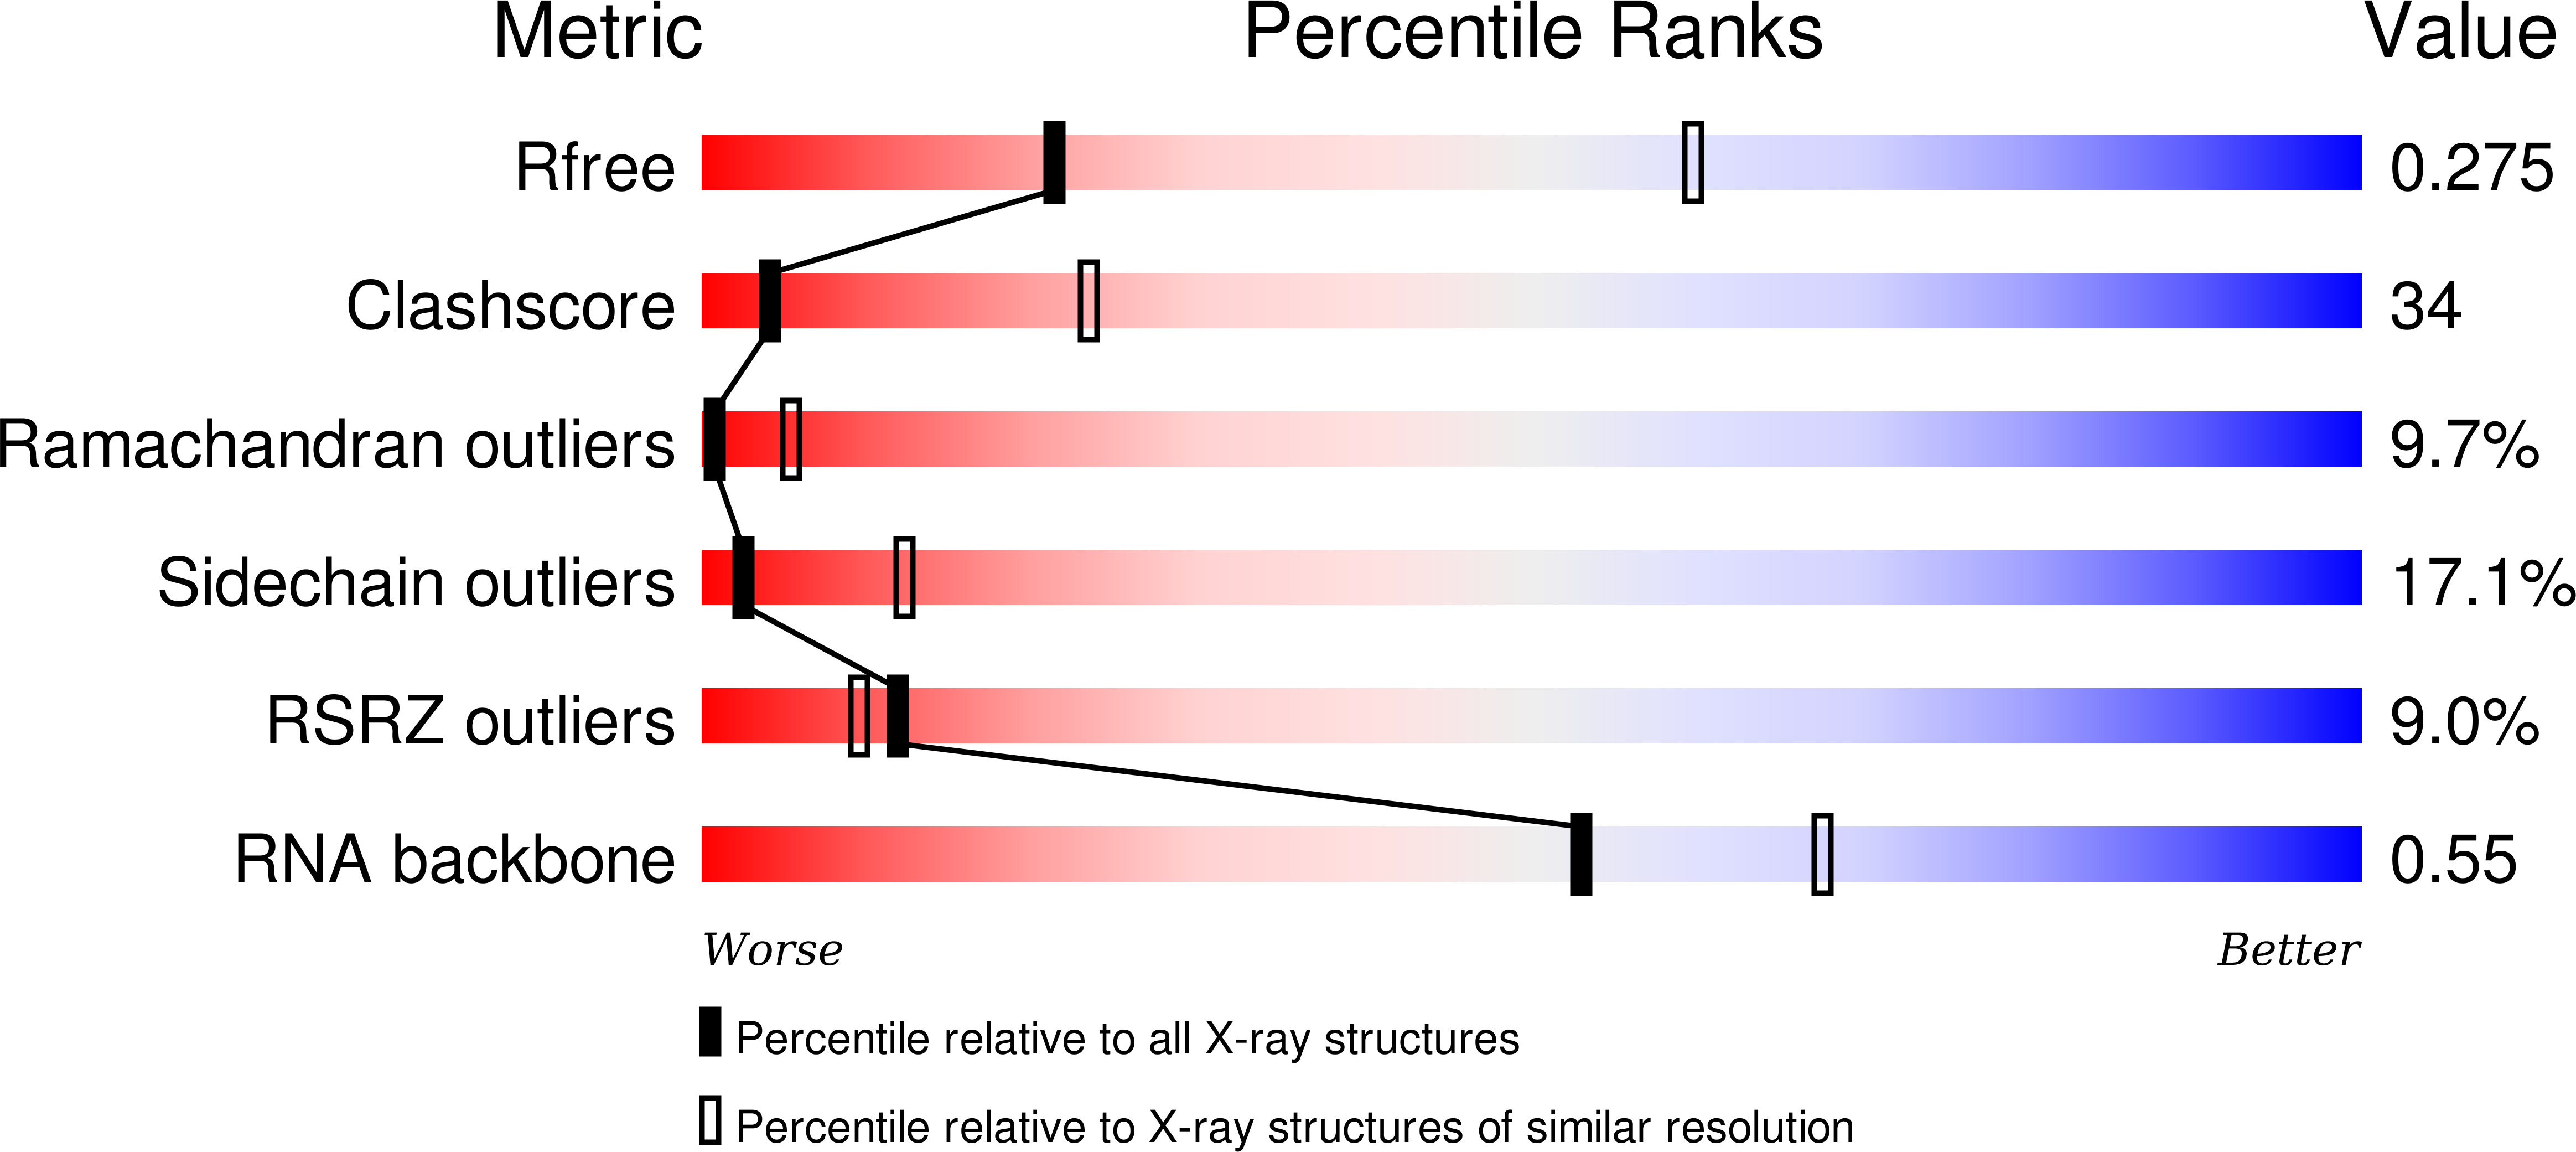
\includegraphics[width=\linewidth]{chapter-4/figs/quality-reports/4V54}
    \caption{4V54}
\label{fig:4V54-quality}
  \end{subfigure}
  \begin{subfigure}[b]{0.5\textwidth}
    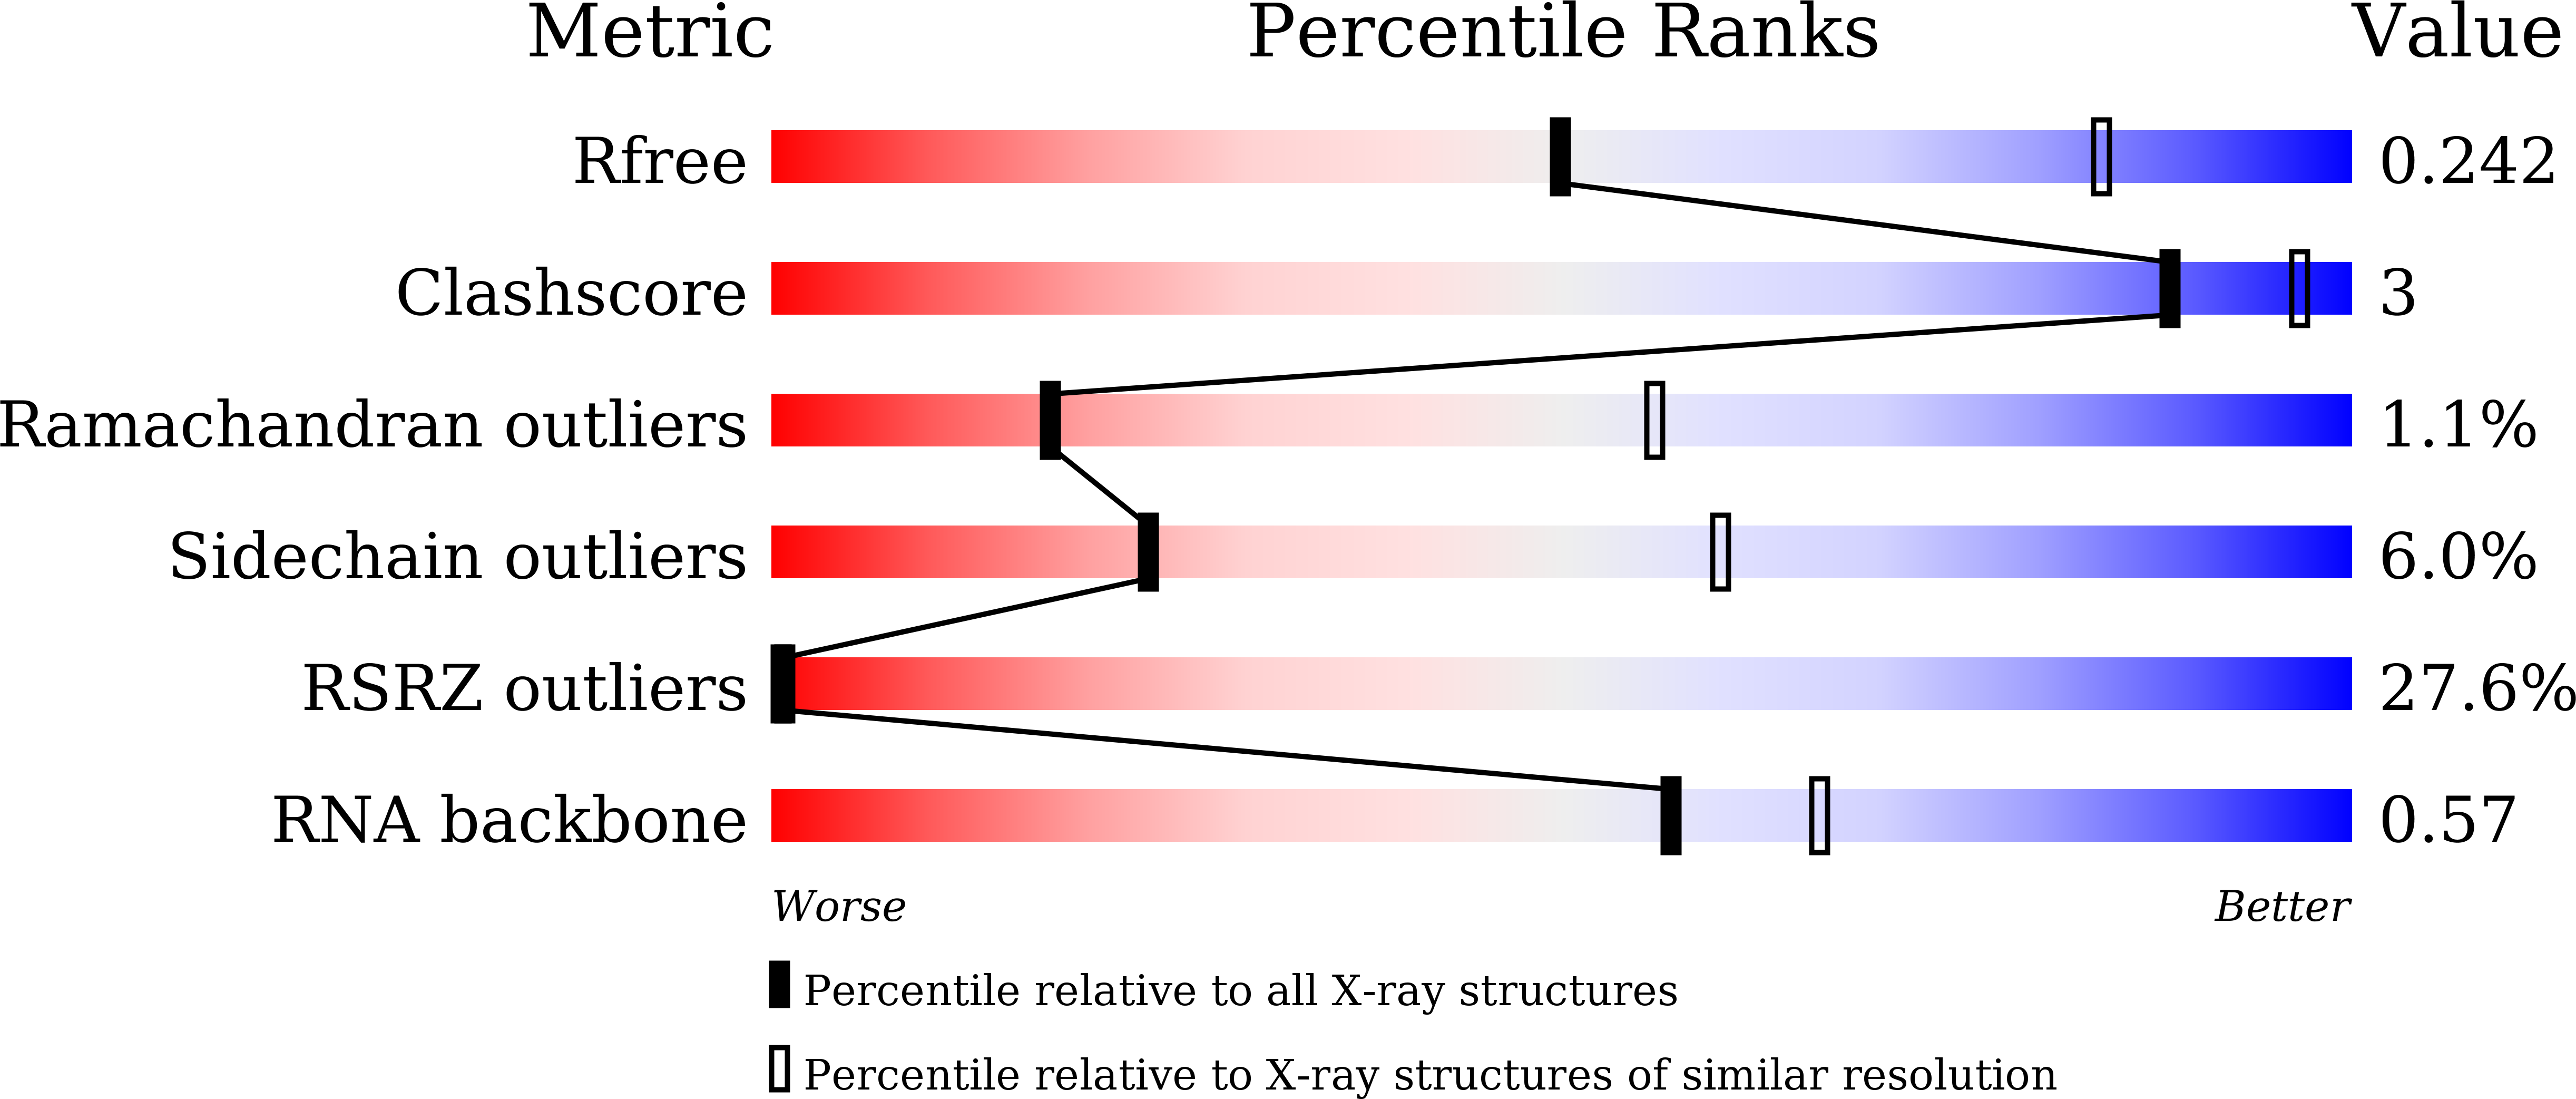
\includegraphics[width=\linewidth]{chapter-4/figs/quality-reports/5J91}
    \caption{5J91}
\label{fig:5J91-quality}
  \end{subfigure}
  \caption{Screenshots of the summaries of quality reports for 4V54 (left), the
    representative selected by the Dual 1\% increase method as compared to the
    report for 5J91 (right), the representative selected by the previous
  method.}
\label{fig:ec-lsu-report}
\end{figure}

The same data is shown for the \TT{} large subunit group in
Figure~\ref{fig:tt-lsu-report}. In this case we see that both structures have
very similar metrics overall. The previous method does select a structure, 5HCQ,
with fewer RSRZ outliers.

\begin{figure}
  \begin{subfigure}[b]{0.5\textwidth}
    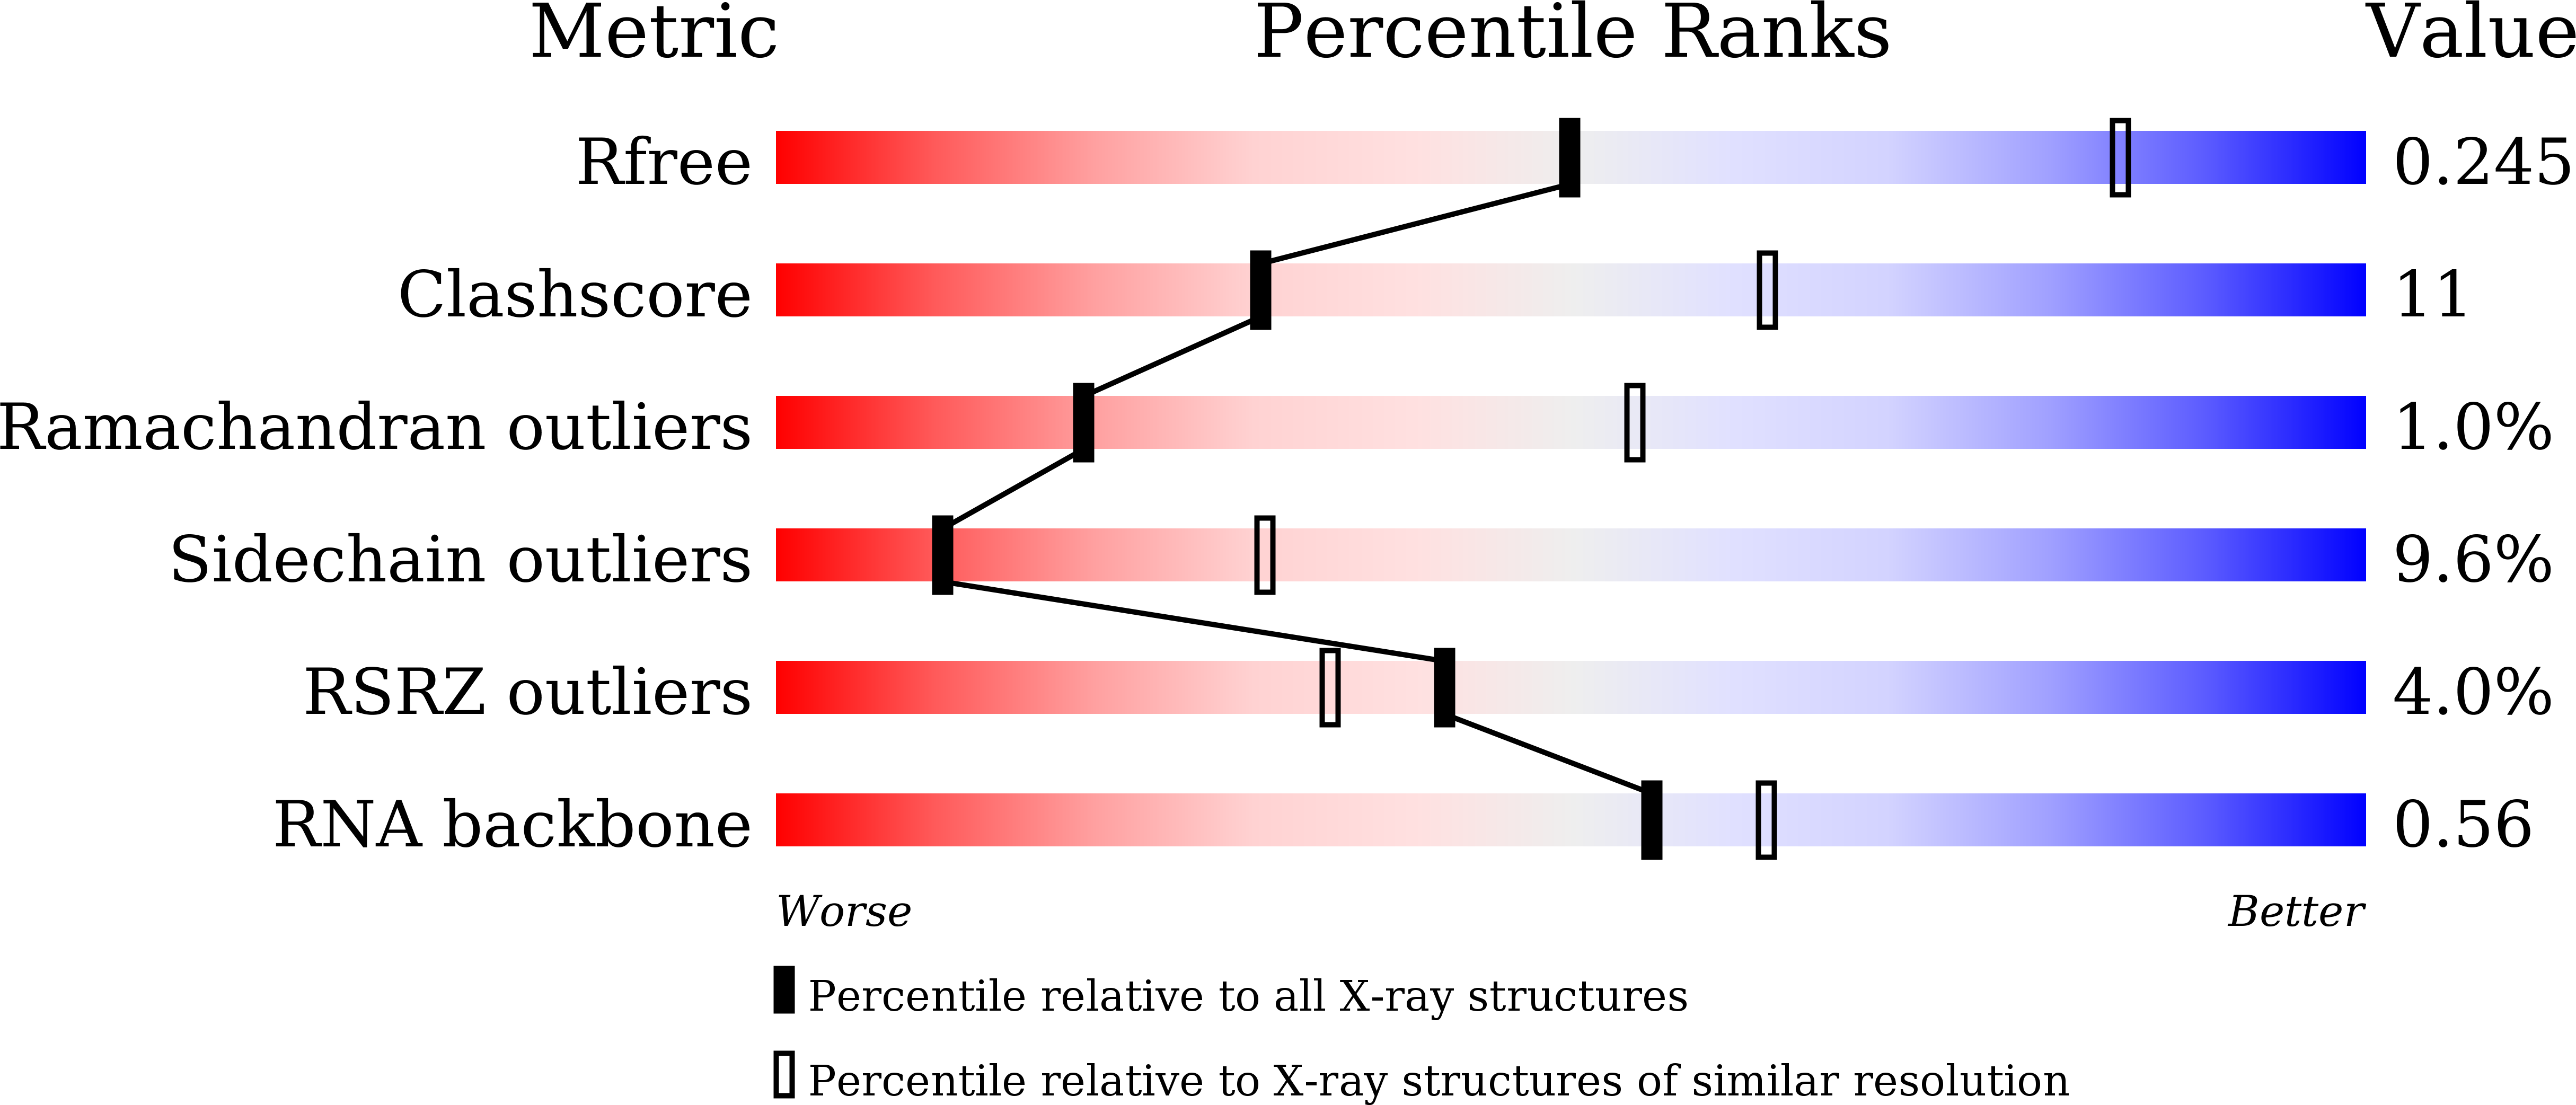
\includegraphics[width=\linewidth]{chapter-4/figs/quality-reports/5FDU}
    \caption{5FDU}
\label{fig:5FDU-quality}
  \end{subfigure}
  \begin{subfigure}[b]{0.5\textwidth}
    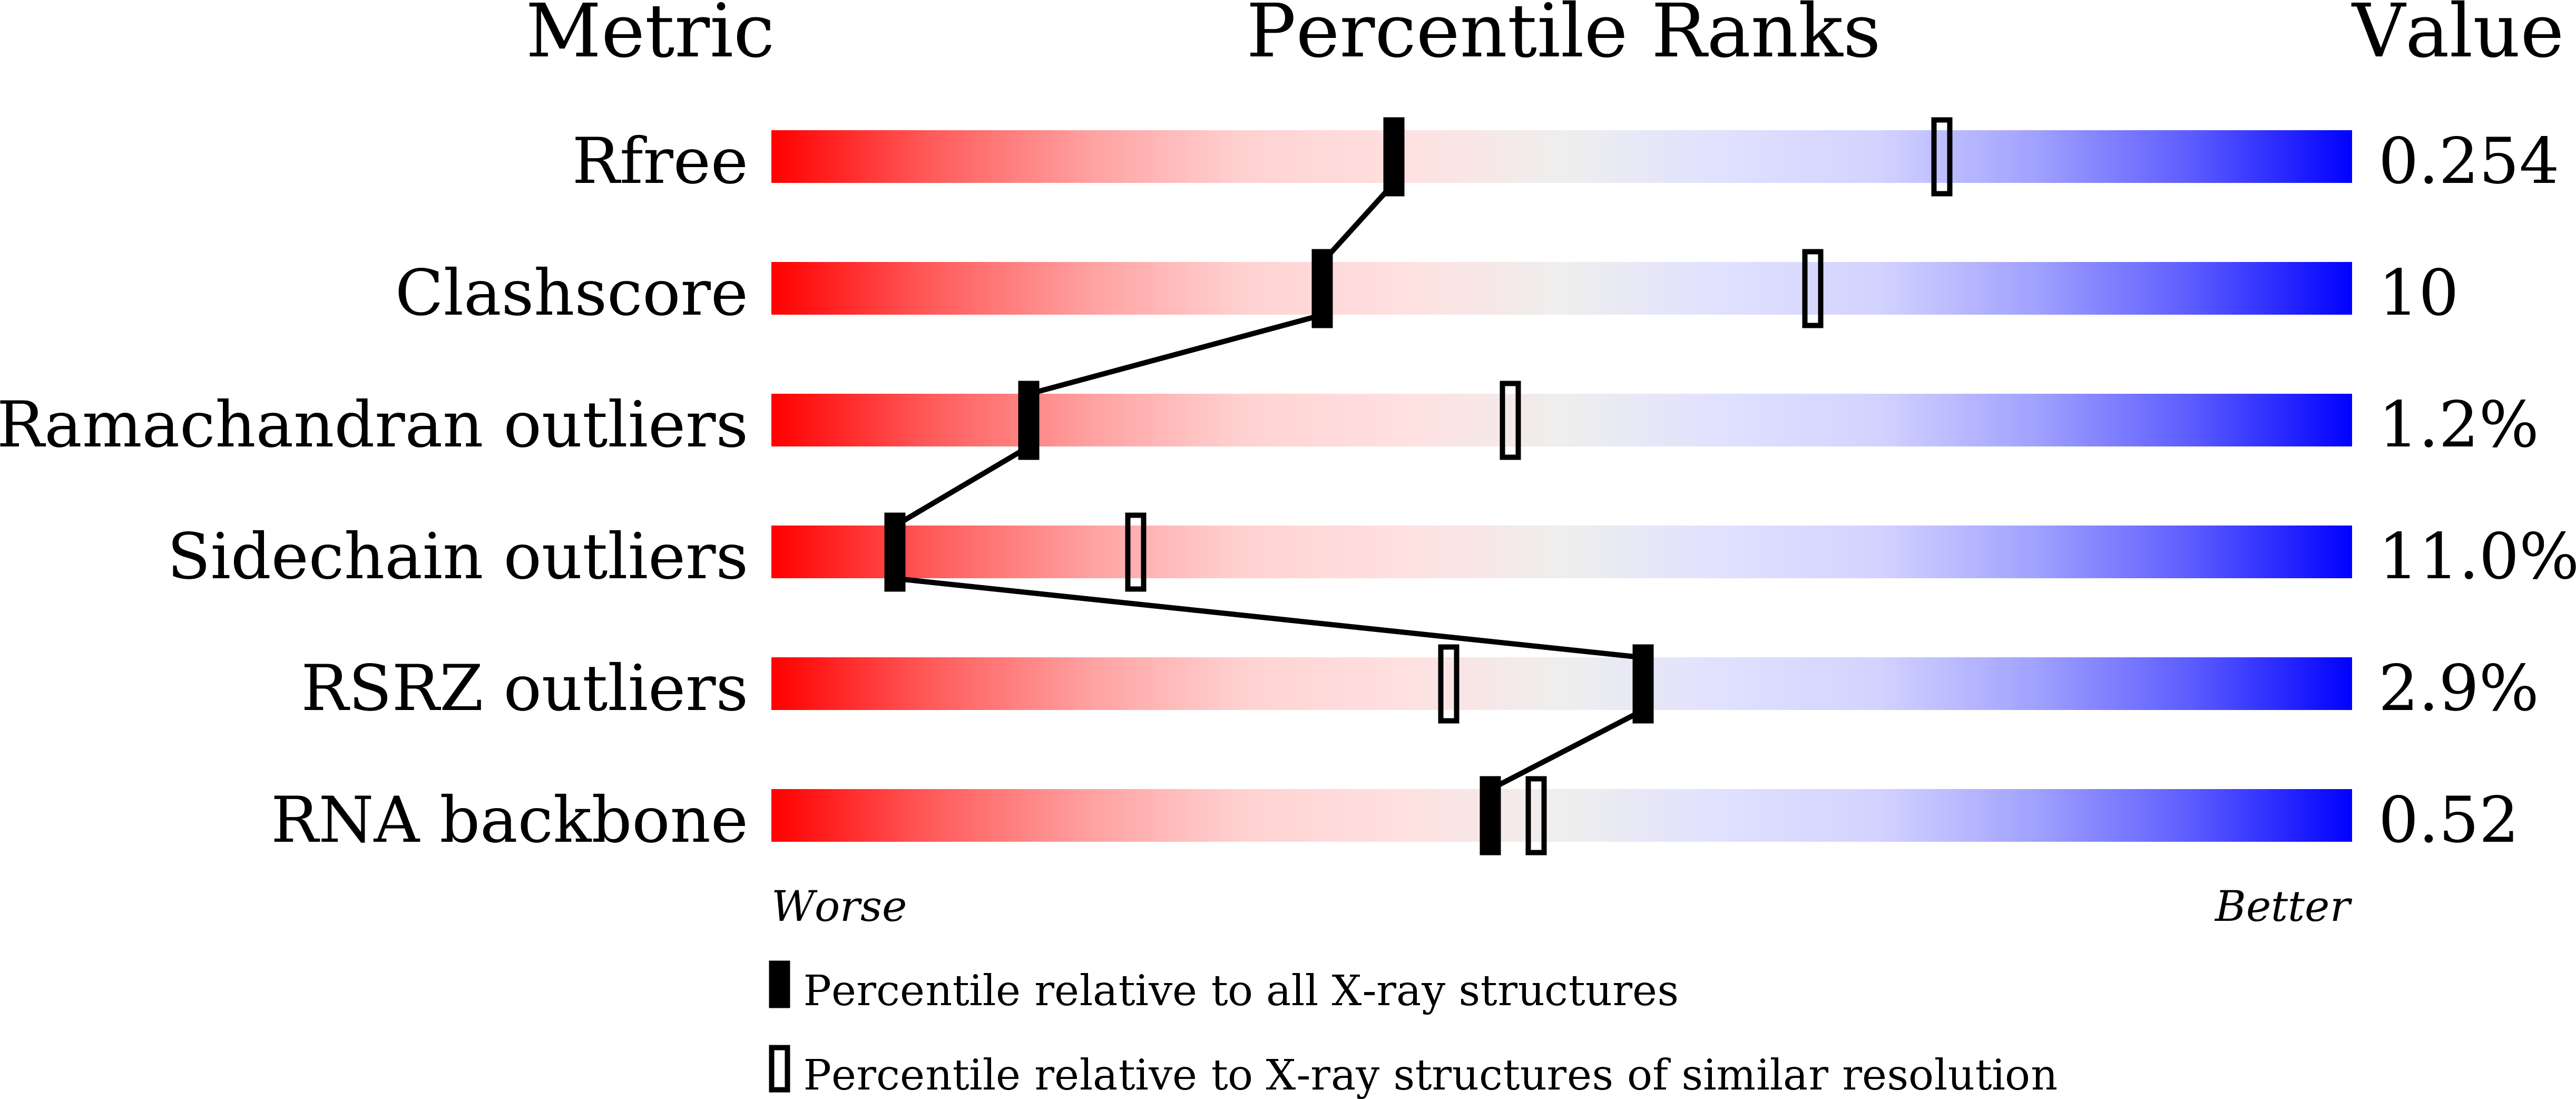
\includegraphics[width=\linewidth]{chapter-4/figs/quality-reports/5HCQ}
    \caption{5HCQ}
\label{fig:5HCQ-quality}
  \end{subfigure}
  \caption{Screenshots of the summaries of quality reports for 5FDU (left), the
          representative selected by the dual 1\% increase method as compared to
          the report for 5HCQ (right), the representative selected by the previous
          method.}
\label{fig:tt-lsu-report}
\end{figure}

These figures indicates that while the dual 1\% increase method does not use the
quality metrics, it does select a good structure.

\subsection{Stability of the Representative Set}

In order to asses the stability of our method we computed the representatives
for a set of 91 weekly releases from 2.0 to 2.90 covering releases from December
5, 2014 to August 26, 2016 using the three methods. We then plotted the number
of changes in the representatives for all equivalence class that are common to
all releases. We expect that the any increase method will be the most unstable,
with the previous and current method being comparable. Our goal is the current
1\% increase method will be more stable. The summary is shown in
Figure~\ref{fig:rep-changes}. This plot summarizes the total number of changes
for 1449 classes that exist in all 91 releases. We can see that all thr% ee
methods are comparable in stability, as they all end near 25 total changes. In
general both the 1\% increase and the previous method are more stable, show fewer
changes, than the any increase method. For most of the plot our current method
shows as many or fewer changes than the previous, indicating it is slightly more
stable.

\begin{figure}
  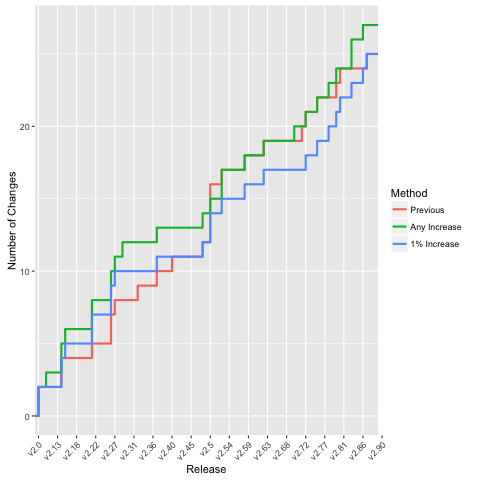
\includegraphics[width=0.5\textwidth]{chapter-4/figs/rep-count-changes}
  \caption{A cumulative distribution of the total number of changes for all
    three methods. This plot is a cumulative sum of the total number changes for
    all classes at the ``all'' resolution cutoff which exist in all of the 90
  releases used in the analysis.}
\label{fig:rep-changes}
\end{figure}

We examined the number of total number of changes for each class in the dataset.
As shown in Table~\ref{tab:rep-changes-count} most classes that exist in all the
releases show no changes. Of those that show changes the majority change only 1
time.

\begin{table}
  \begin{tabular}{lrrrrr}
    \toprule
                        & \multicolumn{5}{c}{Number of Changes} \\
                          \cmidrule(r){2-6}
    Method              & 0    & 1  &  2 &  3 &  4 \\
    \midrule
    Previous Method     & 1528 & 19 &  0 &  2 &  0 \\
    Any Increase Method & 1530 & 17 &  0 &  3 &  0 \\
    1\% Increase Method & 1529 & 16 &  0 &  2 &  1 \\
    \bottomrule
  \end{tabular}
  \caption{Number of changes for classes that exist from 2.0 to 2.90. This table
    summarize the number of classes that show 0, 1, 2, 3, or 4 changes amongst
  the classes that exist in all releases. }
\label{tab:rep-changes-count}
\end{table}

To see how often classes with more than 1 change alters the representative we
plotted all classes that show more than one change across these releases as seen
in Figure~\ref{fig:multi-change}. We see that there are only 3 classes that show
this behavior: 80570, a 2 nucleotide synthetic RNA, 83717 the \EC{} LSU, and
97519 the T\@. t LSU\@. From this we can see that all methods are generally stable
for many releases followed by a few very quick changes. This is more
desirable over a method which changes very frequently. One class, 80570
shown in red, the representative is changed every time a new structure is
added by all methods. This class has few members, 8 in 2.90, and a very
few nucleotides, leading to minor changes in resolution changing the
selected representative. 

\begin{figure}
  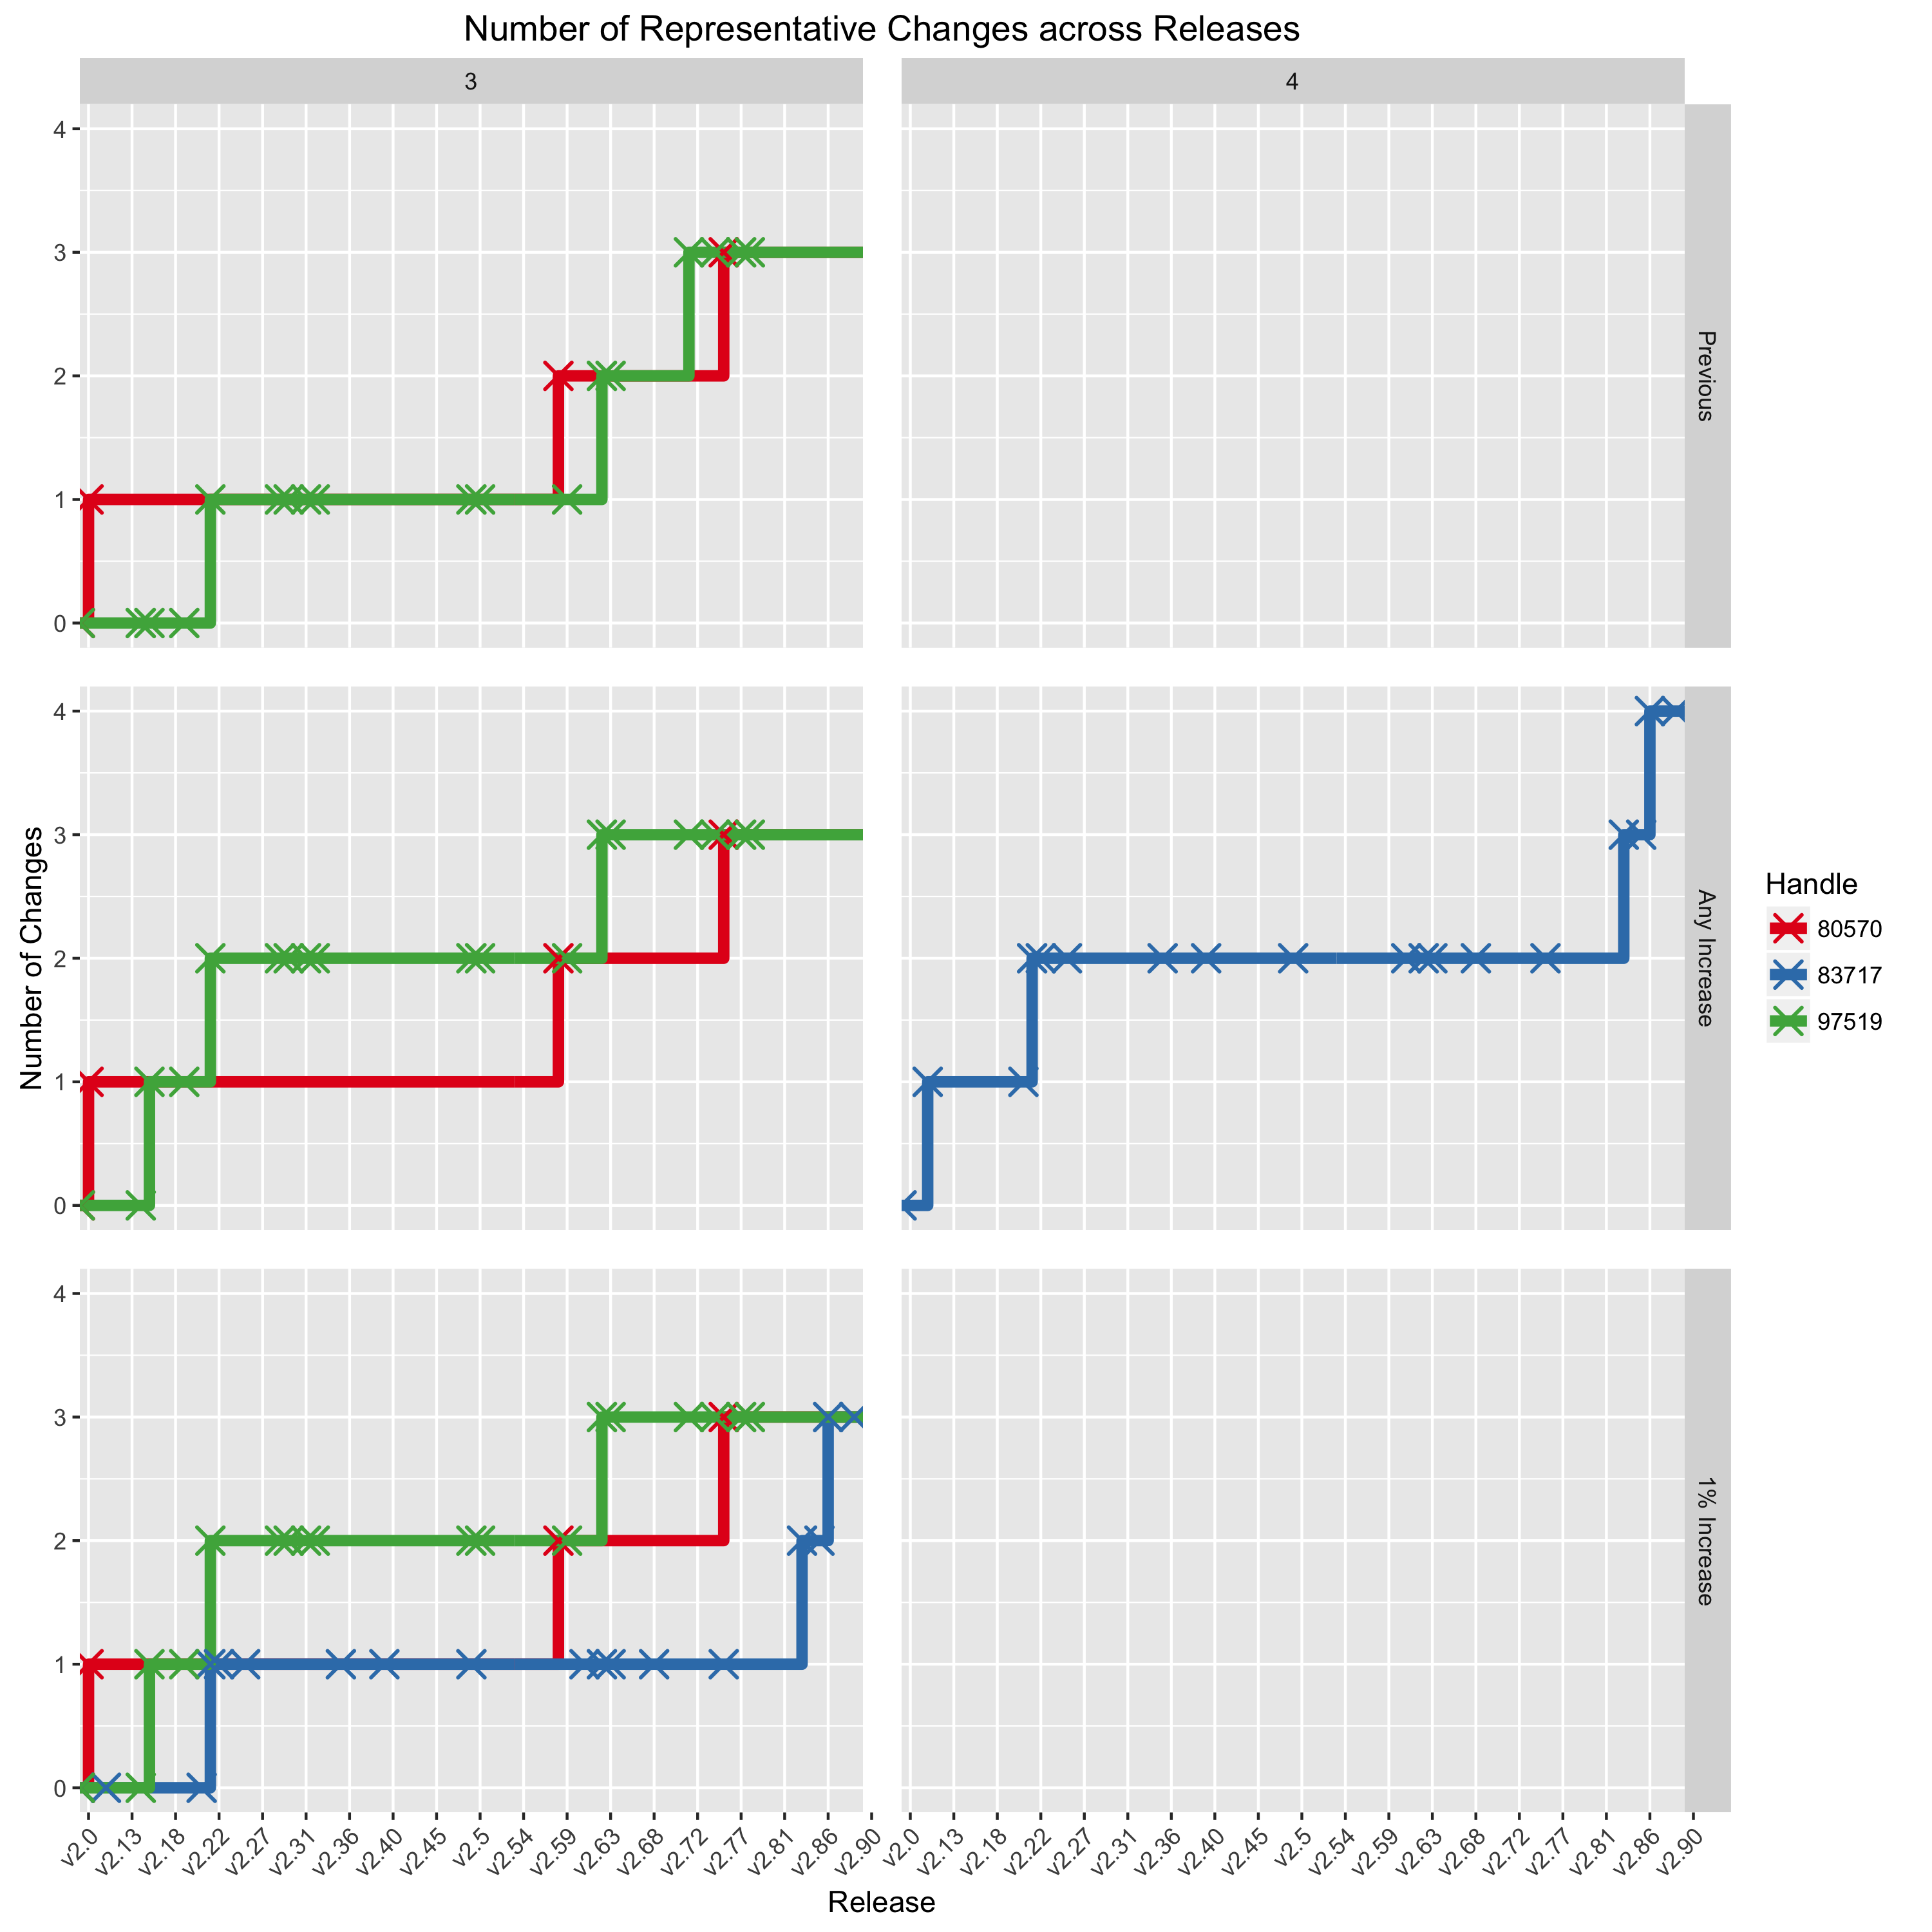
\includegraphics[width=0.5\textwidth]{chapter-4/figs/change-frequency}
  \caption{This figure shows the rate of changes in for each class that changes
    more than once between 2.0 and 2.90. Each colored line represents a class,
    and each mark indicates when members are added to the class. The three sets
  panels indicate the three different methods tested here.}
\label{fig:multi-change}
\end{figure}

\section{Conclusions and future work}

In summary, we have developed a method to select a representative structure from
our equivalence classes. This method reliably selects a good structure from the
set of structures. It is also stable and will not change due to small
improvements in the structure.

One possible improvement is to use the quality metrics provided by PDB, such as
real space refinement (RSR) and the RSR Z-score (RSRZ) in the selection of the
representative structure. These are measures of how well a modeled structure
fits the underlying data from the experiment. This data and its utility will be
discussed in detail in the following chapter. Usage of this data will allow us
to detect if a structure is well modeled. This could be used in place of our
base pairs per nucleotides metric to select structures. The downside is that not
all structures have RSRZ data. Notably, cyro-em structures do not yet have such
a metric. The community is working on such metrics however.
